\documentclass[beamer,10pt,fleqn]{beamer}

%\setbeamercovered{transparent}

\usepackage{xcolor}
\usepackage{graphicx}
\usepackage{amssymb}
\usepackage{amsfonts}
\usepackage{amsmath}
\usepackage{multirow}
\usepackage{tikz}
\usepackage{pgfplots}
%\usepackage{gnuplot-lua-tikz}
\usepackage{minibox}
\usepackage{booktabs}

\usetikzlibrary{shapes,shapes.multipart,arrows,chains}
\usepackage{fancyvrb}
\usepackage{listings}
\usetikzlibrary{spy}
\usepackage{amssymb}
\usepackage{alltt}
\usepackage{proof}
\usepackage{wrapfig}
\usepackage{etoolbox}
\usepackage{cancel}

\definecolor{cola}{rgb}{0.878431, 0.235294, 0.192157}
\definecolor{colb}{rgb}{0.552941, 0.72549, 0.792157}
\definecolor{colc}{rgb}{0.964706, 0.745098, 0}
\definecolor{cold}{rgb}{0.643137, 0.758824, 0.809804}
\definecolor{cole}{rgb}{0.54902, 0.509804, 0.47451}
\definecolor{colf}{rgb}{0.917647, 0.462745, 0}
\definecolor{colg}{rgb}{0.141176, 0.313725, 0.603922}
\definecolor{colh}{rgb}{0.709804, 0.741176, 0}
\definecolor{coli}{rgb}{0.835294, 0, 0.196078}
\definecolor{colj}{rgb}{0, 0.592157, 0.662745}
\definecolor{colk}{rgb}{0.67451, 0.0784314, 0.352941}
\definecolor{coll}{rgb}{0.333333, 0.313725, 0.145098}
\definecolor{colm}{rgb}{0.396078, 0.113725, 0.196078}
\definecolor{coln}{rgb}{0.294118, 0.219608, 0.298039}
\definecolor{colo}{rgb}{0, 0.239216, 0.298039}
\definecolor{colp}{rgb}{0.305882, 0.211765, 0.160784}
\definecolor{colq}{rgb}{0.560784, 0.6, 0.243137}
\definecolor{colr}{rgb}{0.576471, 0.152941, 0.172549}
\definecolor{cols}{rgb}{0.313725, 0.027451, 0.470588}
\definecolor{colt}{rgb}{0, 0.156863, 0.333333}
\definecolor{colu}{rgb}{0.776471, 0.690196, 0.737255}
\definecolor{colv}{rgb}{0.733333, 0.772549, 0.572549}
\definecolor{colw}{rgb}{0.139216, 0.123529, 0.268627}




\newcommand{\colaa}{darkpurple} %1
\newcommand{\colab}{midgreen!60!brightgreen} %2
\newcommand{\colac}{midblue} %3
\newcommand{\colad}{clearorange} %4
\newcommand{\colae}{redorange} %5
\newcommand{\colaf}{clearyellow} %6
\newcommand{\colag}{midyellow!80!redorange} %7

\newcommand{\numa}{\textcolor{white}{${1}$}}
\newcommand{\numb}{\textcolor{white}{${2}$}}
\newcommand{\numc}{\textcolor{white}{${3}$}}
\newcommand{\numd}{\textcolor{white}{${4}$}}
\newcommand{\nume}{\textcolor{white}{${5}$}}
\newcommand{\numf}{\textcolor{white}{${6}$}}
\newcommand{\numg}{\textcolor{white}{${7}$}}
\newcommand{\colah}{midgreen}
\newcommand{\numh}{\textcolor{white}{${8}$}}
\newcommand{\colai}{darkturqoise!70!white}
\newcommand{\numi}{\textcolor{white}{$9$}}
\newcommand{\colaj}{darkred}
\newcommand{\numj}{\textcolor{white}{$\!{10}\!$}}
\newcommand{\colak}{lightpurple}
\newcommand{\numk}{\textcolor{white}{$\!{11}\!$}}
\newcommand{\colal}{lightblue}
\newcommand{\numl}{\textcolor{white}{$\!{12}\!$}}
\newcommand{\colam}{greypurple!70!white}
\newcommand{\numm}{\textcolor{white}{$\!{13}\!$}}
\newcommand{\colan}{softgreen}
\newcommand{\numn}{\textcolor{white}{$\!{14}\!$}}

\newcommand{\onesquare}[5]{
 	\node[fill=#3, opacity=1, minimum width=#5, minimum height=#5] (#1#2) at (#1, #2) {#4};
 }
 
  \newcommand{\dashedonesquare}[4]{
 	\node[fill=#3, opacity=1, minimum width=#4, minimum height=#4] (#1#2) at (#1, #2) {};
    \draw (#1-0.25, #2-0.25) -- (#1 + 0.25, #2 + 0.25);
    \draw (#1+0.25, #2-0.25) -- (#1 - 0.25, #2 + 0.25);
 }

\usepackage{euler}
\def\mathfamilydefault{\rmdefault}

\newcommand{\myitemsep}{
    \setlength{\itemsep}{5pt}
    \setlength{\parskip}{0pt}
    \setlength{\parsep}{0pt}
    \vspace{3pt}
}

\newenvironment{myitemize}{\begin{itemize}\myitemsep}{\end{itemize}}
\newenvironment{myenumerate}{\begin{enumerate}\myitemsep}{\end{enumerate}}
\newenvironment{myqenumerate}{\begin{enumerate}[(Q1)]\myitemsep}{\end{enumerate}}

\def\L#1{\raise .2ex\hbox{\tiny\tt #1}&}
\def\C#1{\mbox{\bf//}\ \small\relax#1}
\def\S#1{\mbox{\emph{#1}}}
\def\K#1{\textbf{#1}}
\def\N{\\[.9ex]}                                      
\def\I{\hspace{1em}}

\definecolor{fillcolor}{rgb}{0.5, 0.5, 0.5} 
\definecolor{drawcolor}{rgb}{0, 0, 0} 
\tikzstyle{grayfill} = [fill=fillcolor!70, draw=drawcolor, thick]
\tikzstyle{whitefill} = [fill=white, draw=drawcolor, thick] 


\newcommand{\NN}{\mathbb{N}}
\newcommand{\Pat}{\mathrm{AT}}
\newcommand{\Prat}{\mathrm{RAT}}

\newcommand{\upone}{\vdash_1}
\newcommand{\emptys}{\epsilon}

\usecolortheme[RGB={196, 30, 58}]{structure}
\tikzstyle{every circle node}=[circle,inner sep=1.5pt,minimum size=0.4cm]


\definecolor{xred}{rgb}{.7 .1 .1}
\definecolor{xpurple}{rgb}{.7 .3 .5}

\definecolor{xgreen}{rgb}{.0 .5 .0}
\definecolor{royalred}{rgb}{.9 .1 .3}
\definecolor{royalgreen}{rgb}{.2 .7 .4}

\definecolor{xorange}{cmyk}{0,0.65,1,0.09}
%\definecolor{xgreen}{rgb}{0.66, 0.77, 0.5}
\definecolor{xblue}{rgb}{0., 0.25, 1}

\newcommand{\lneg}{\bar}

\newcommand{\plit}[1]{\only<2>{\textcolor{royalgreen}}{x_{#1}}}
\newcommand{\qlit}[1]{\only<2>{\textcolor{royalred}}{x_{#1}}}
\newcommand{\nlit}[1]{\only<2>{\textcolor{royalred}}{\overline x_{#1}}}
\newcommand{\mlit}[1]{\only<2>{\textcolor{royalgreen}}{\lnot x_{#1}}}


\tikzstyle{every star node}=[star,star points=6,draw,inner sep=1.5pt,minimum size=0.3cm,fill=yellow]

\newrobustcmd*{\mysquare}[1]{\tikz{\filldraw[draw=#1,fill=#1] (0,0) rectangle (0.2cm,0.2cm);}}
%\newrobustcmd*{\mycircle}[0]{\tikz{\filldraw[draw=black,fill=none] (0,0) circle [radius=0.125cm];}}
\newrobustcmd*{\mycircle}[0]{F}
\newrobustcmd*{\mytriangle}[0]{\tikz{\filldraw[draw=black,fill=none] (0,0) -- (0.2cm,0) -- (0.1cm,0.2cm) -- (0,0) --  (0.2cm,0);}}

%\DeclareMathOperator{\var}{var}

\lstdefinestyle{CPlain}{ %
basicstyle=\scriptsize\ttfamily, % the size of the fonts 
numbers=left,                   % where to put the line-numbers
numberstyle=\tiny,      % the size of the fonts that are used for th
stepnumber=1,                   % the step between two line-numbers
numbersep=5pt,                  % how far the line-numbers are from the code
backgroundcolor=\color{white},  % choose the background color
showspaces=false,               % show spaces adding particular underscores
showstringspaces=false,         % underline spaces within strings
showtabs=false,                 % show tabs within strings adding 
frame=single,           % adds a frame around the code
tabsize=2,          % sets default tabsize to 2 spaces
captionpos=b,           % sets the caption-position to bottom
breaklines=true,        % sets automatic line breaking
breakatwhitespace=false,    % sets if automatic breaks should only happen
fancyvrb=true,
}

\newenvironment{CodePlain}[1][]
  { \VerbatimEnvironment%
    \begin{Verbatim}[#1]}
  { \end{Verbatim}  } 

\setbeamertemplate{footline}
{
	\leavevmode%
	\hbox{%
	\begin{beamercolorbox}[wd=0.35\paperwidth,ht=2.25ex,dp=1ex,center]{author in head/foot}%
	\small {Happy Ending Problem}
%        \small {Logic and Mechanized Reasoning}
			\vspace{4pt}
	\end{beamercolorbox}%
	\begin{beamercolorbox}[wd=0.45\paperwidth,ht=2.25ex,dp=1ex,center]{author in head/foot}%
	\end{beamercolorbox}%
	\begin{beamercolorbox}[wd=0.2\paperwidth,ht=2.5ex,dp=1ex,right]{date in head/foot}%
		\structure{\scriptsize \insertframenumber{} / \inserttotalframenumber\hspace*{3ex}}
		\vspace{3pt}
	\end{beamercolorbox}}%
	\vskip0pt%
}

\beamertemplatenavigationsymbolsempty

\title{Automated Reasoning Exciting Challenges\\ \huge Happy Ending Problem}

\author[Marijn Heule]{{\bf \large Marijn J.H. Heule}\\[5pt] joint work with Manfred Scheucher}

\institute[CMU and AWS]{
\includegraphics[height=50pt]{images/CMU_Logo}~~~~~~~~
\includegraphics[height=50pt]{images/scholars}}

\date{Automated Reasoning Reading Group\\September 1, 2023}

%\date{Simons Institute~~~~~~~April 3, 2023}
%\date{}


%\institute[CMU]{
\includegraphics[height=50pt]{figures/CMU_Logo}}

\definecolor{xblue}{rgb}{0., 0.25, 1}

\newcommand{\vertex}[3]{
  \draw[fill=blue] (#1, #2) circle (#3 pt);
}

\newcommand{\vertexc}[4]{
  \draw[fill=#4] (#1, #2) circle (#3 pt);
}

\begin{document}


\begin{frame}
    \titlepage
\end{frame}

\section{Introduction}
\frame{\Large \tableofcontents[currentsection]}

\frame{
	\frametitle{Points in General Position}

\large

A finite point set \structure{$S$} in the plane is
in \structure{general position} if no three points in $S$ are on a line.

\medskip
	
\begin{center}
\begin{tikzpicture}[scale=0.25]
\vertex{13.52465}{62.02656}{6};
\vertex{19.8803}{64.71728}{6};
\vertex{36.07544}{71.57344}{6};
  \draw[shift={(11.2695, 61.0718)}, rotate=-15.4222, scale=1.2, thick]
    (0, 0)
     -- (19.2, 15.2);
  \draw[shift={(22.723, 69.8435)}, scale=0.6, structure, line width=3pt]
    (0, 0)
     -- (11.2, -11.2);
  \draw[shift={(22.2124, 62.3084)}, scale=0.6, structure, line width=3pt]
    (0, 0)
     -- (11.2, 13.6);
\end{tikzpicture}
\end{center}

\bigskip
\bigskip
\pause

\centering

\structure{throughout this talk, every set is in general position}

}


\frame{
	\frametitle{Erd\H{o}s–Szekeres Numbers}
	
\large 

A \structure{$k$-gon} (in S) is the vertex set of a convex $k$-gon

\bigskip

\begin{center}
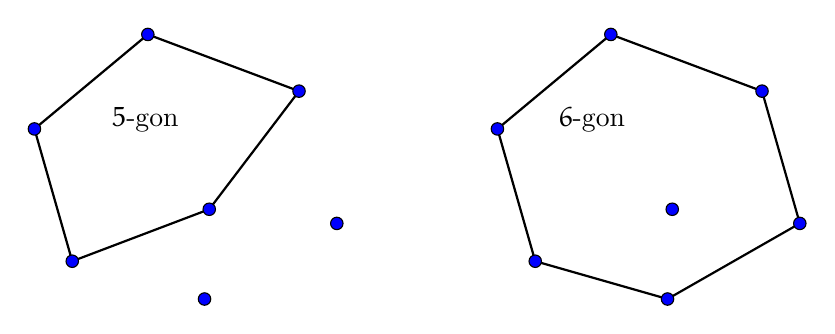
\begin{tikzpicture}[scale=1.5]
\newcommand\x{1.5}
  \draw[thick]
    (-.56, 3.48)
     -- (.40, 4.28)
     -- (1.68, 3.80)
     -- (.92, 2.80)
     -- (-.24, 2.36)
     -- (-.56, 3.48);
\vertex{-.56}{3.48}{\x};
\vertex{.40}{4.28}{\x};
\vertex{1.68}{3.80}{\x};
\vertex{2.00}{2.68}{\x};
\vertex{.88}{2.04}{\x};
\vertex{.92}{2.80}{\x};
\vertex{-.24}{2.36}{\x};
  \draw[thick]
    (3.68, 2.36)
     -- (3.36, 3.48)
     -- (4.32, 4.28)
     -- (5.60, 3.80)
     -- (5.92, 2.68)
     -- (4.80, 2.04)
     -- (3.68, 2.36);
\vertex{3.36}{3.48}{\x};
\vertex{4.32}{4.28}{\x};
\vertex{5.60}{3.80}{\x};
\vertex{5.92}{2.68}{\x};
\vertex{4.80}{2.04}{\x};
\vertex{4.84}{2.80}{\x};
\vertex{3.68}{2.36}{\x};
  \node
     at (.38, 3.56) {$5$-gon};
  \node
     at (4.16, 3.56) {$6$-gon};
\end{tikzpicture}
\end{center}

\begin{theorem}[Erd\H{o}s \& Szekeres 1935]
$\forall k \in \mathbb{N}, \exists$ a smallest integer $g(k)$ such that every set of $g(k)$ points contains a $k$-gon.
\end{theorem}

}

\frame{
	\frametitle{Bounds for Small $k$}

\large 

Clearly, it takes exactly three points in general position to have a $3$-gon (triangle)


\bigskip

Some sets of 4 points do not for a $4$-gon:

\bigskip

\centering

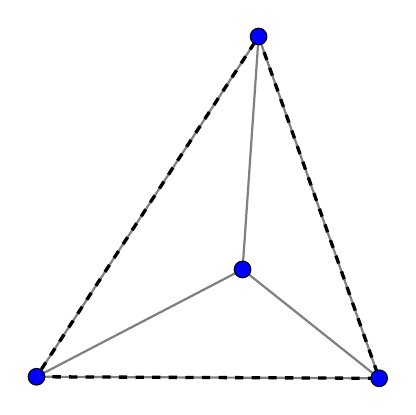
\begin{tikzpicture}[scale=1.5]
\newcommand{\x}{2}

  \draw [gray, thick] (0.423016, 4.503319) -- (2.303165, 7.383978);
  \draw [gray, thick] (0.423016, 4.503319) -- (3.32398, 4.490406);
  \draw [gray, thick] (0.423016, 4.503319) -- (2.167452, 5.411797);

  \draw [gray, thick] (3.32398, 4.490406) -- (2.303165, 7.383978);
  \draw [gray, thick] (2.167452, 5.411797) -- (3.32398, 4.490406);
  \draw [gray, thick] (2.303165, 7.383978) -- (2.167452, 5.411797);

  \draw[dashed, very thick]
    (2.30317, 7.38398)
     -- (3.32398, 4.490406)
     -- (0.42302, 4.503321)
     -- cycle;

\vertex{0.423016}{4.503319}{\x};
\vertex{2.303165}{7.383978}{\x};
\vertex{2.167452}{5.411797}{\x};
\vertex{3.32398}{4.490404}{\x};

\end{tikzpicture}

\bigskip

\pause



\structure{how many points imply a $4$-gon?}



}

\frame{
	\frametitle{Upperbound for $4$-Gon: $g(4) = 5$ \textcolor{xgreen}{[Klein]}}

\large

   \newcommand{\x}{0.75}


\centering
	
	
\begin{tikzpicture}[scale=2.5]

  \draw[shift={(1, 3.04)}, scale=1.5, thick]
    (0, 0)
     -- (0.64, 0.32)
     -- (1.12, 0)
     -- (0.8, -0.48)
     -- (0.32, -0.48)
     -- cycle;

\only<2->{
  \filldraw[shift={(1, 3.04)}, scale=1.5, draw=structure, very thick, fill=structure!30!white]
    (0, 0)
     -- (0.64, 0.32)
     -- (1.12, 0)
 %    -- (0.8, -0.48)
     -- (0.32, -0.48)
     -- cycle;     
}
     
  \vertex{2.2}{2.32}{\x};
  \vertex{2.68}{3.04}{\x};
  \vertex{1.96}{3.52}{\x};
  \vertex{1}{3.04}{\x};
  \vertex{1.48}{2.32}{\x};

\end{tikzpicture}
~~~~~~~~~~~~~~~~~~~~
\pause
\pause
\begin{tikzpicture}[scale=2.5]
  \draw[shift={(3.8, 2.32)}, scale=1.5, thick]
    (0, 0)
     -- (0, 0.8)
     -- (0.8, 0.64)
     -- (0.64, 0.16)
     -- cycle;

%  \draw[shift={(3.8, 3.52)}, scale=1.5]
%    (0, 0)
%     -- (0.64, -0.64);
%  \draw[shift={(3.8, 2.32)}, scale=1.5]
%    (0, 0)
%     -- (0.8, 0.64);

\only<4->{
  \filldraw[shift={(3.8, 3.52)}, scale=1.5, draw=structure, very thick, fill=structure!30!white]
    (0, 0)
     -- (0.16, -0.48)
     -- (0.64, -0.64)
     -- (0.8, -0.16)
     -- cycle;
     
%   \draw[shift={(3.8, 3.52)}, scale=1.5]
%    (0, 0)
%     -- (0.64, -0.64);
%  \draw[shift={(3.8, 2.32)}, scale=1.5]
%    (0, 0)
%     -- (0.8, 0.64);
}

  \vertex{4.04}{2.8}{\x};
  \vertex{3.8}{3.52}{\x};
  \vertex{5}{3.28}{\x};
  \vertex{4.76}{2.56}{\x};
  \vertex{3.8}{2.32}{\x};

\end{tikzpicture}

\pause
\pause
	
\begin{tikzpicture}[scale=2.5]
     
  
    \draw[shift={(5.72, 2.56)}, scale=1.5]
    (0, 0)
     -- (1.28, 0.48);

  \draw[shift={(5.96, 2.32)}, scale=1.5, thick]
    (0, 0)
     -- (0.48, 0.96)
     -- (0.96, 0.16)
     -- cycle;

\only<6->{

    \draw[shift={(5.72, 2.56)}, scale=1.5]
    (0, 0)
     -- (1.28, 0.48);
     
  \filldraw[shift={(5.96, 2.32)}, scale=1.5, draw=structure, very thick, fill=structure!30!white]
    (0, 0)
     -- (0.3426, 0.348475)
     -- (0.59104, 0.44164)
     -- (0.96, 0.16)
     -- cycle;
 }
 
  \vertex{6.4739}{2.842713}{\x};
  \vertex{6.84656}{2.98246}{\x};
  \vertex{5.96}{2.32}{\x};
  \vertex{6.68}{3.76}{\x};
  \vertex{7.4}{2.56}{\x};
  

  \end{tikzpicture}	

}

\frame{
	\frametitle{Bound Results for $5$-Gon and $6$-Gon}


\begin{minipage}{0.45\textwidth}
$g(5) = 9$
\begin{itemize}
\item \textcolor{xgreen}{[Kalbfleisch \& Stanton '70]}
\end{itemize}
\end{minipage}
\begin{minipage}{0.45\textwidth}
\centering
\medskip
~~~~~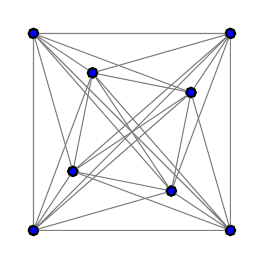
\begin{tikzpicture}[scale=0.5]

\node[draw,circle, thick, fill=blue, scale=0.3] (a) at (0,0) {};
\node[draw,circle, thick, fill=blue, scale=0.3] (b) at (5,0) {};
\node[draw,circle, thick, fill=blue, scale=0.3] (c) at (0,5) {};
\node[draw,circle, thick, fill=blue, scale=0.3] (d) at (5,5) {};

\node[draw,circle, thick, fill=blue, scale=0.3] (e) at (1,1.5) {};
\node[draw,circle, thick, fill=blue, scale=0.3] (f) at (3.5,1) {};
\node[draw,circle, thick, fill=blue, scale=0.3] (g) at (1.5,4) {};
\node[draw,circle, thick, fill=blue, scale=0.3] (h) at (4,3.5) {};

\draw[gray] (a) -- (b) (a) -- (c) (a) -- (d) (a) -- (e) (a) -- (f) (a) -- (g) (a) -- (h);
\draw[gray] (b) -- (c) (b) -- (d) (b) -- (e) (b) -- (f) (b) -- (g) (b) -- (h);
\draw[gray] (c) -- (d) (c) -- (e) (c) -- (f) (c) -- (g) (c) -- (h);
\draw[gray] (d) -- (e) (d) -- (f) (d) -- (g) (d) -- (h);
\draw[gray] (e) -- (f) (e) -- (g) (e) -- (h);
\draw[gray] (f) -- (g) (f) -- (h)  (g) -- (h);
 
\end{tikzpicture}
\end{minipage}


\begin{minipage}{0.45\textwidth}
\centering
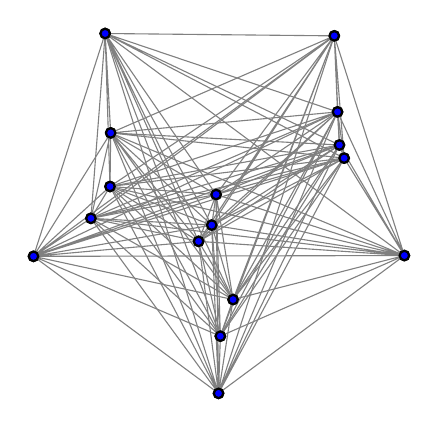
\begin{tikzpicture}[scale=1]

\node[draw,circle, thick, fill=blue, scale=0.3] (a) at (0.19, 1.95) {};
\node[draw,circle, thick, fill=blue, scale=0.3] (b) at (2.54, 0.21) {};
\node[draw,circle, thick, fill=blue, scale=0.3] (c) at (4.9, 1.96) {};
\node[draw,circle, thick, fill=blue, scale=0.3] (d) at (4.01, 4.75) {};
\node[draw,circle, thick, fill=blue, scale=0.3] (e) at (1.1, 4.78) {};
\node[draw,circle, thick, fill=blue, scale=0.3] (f) at (2.5091, 2.735) {};
\node[draw,circle, thick, fill=blue, scale=0.3] (g) at (1.1702, 3.5174) {};
\node[draw,circle, thick, fill=blue, scale=0.3] (h) at (4.0512, 3.7842) {};
\node[draw,circle, thick, fill=blue, scale=0.3] (i) at (2.7243, 1.4014) {};
\node[draw,circle, thick, fill=blue, scale=0.3] (j) at (0.9192, 2.4327) {};
\node[draw,circle, thick, fill=blue, scale=0.3] (k) at (4.1349, 3.1973) {};
\node[draw,circle, thick, fill=blue, scale=0.3] (l) at (2.2864, 2.1402) {};
\node[draw,circle, thick, fill=blue, scale=0.3] (m) at (2.5628, 0.9363) {};
\node[draw,circle, thick, fill=blue, scale=0.3] (n) at (1.1617, 2.8371) {};
\node[draw,circle, thick, fill=blue, scale=0.3] (o) at (2.4537, 2.3468) {};
\node[draw,circle, thick, fill=blue, scale=0.3] (p) at (4.0752, 3.364) {};
 
 
\draw[gray] (a) -- (b) (a) -- (c) (a) -- (d) (a) -- (e) (a) -- (f) (a) -- (g) (a) -- (h) (a) -- (i) (a) -- (j) (a) -- (k) (a) -- (l) (a) -- (m) (a) -- (n) (a) -- (o) (a) -- (p);
\draw[gray] (b) -- (c) (b) -- (d) (b) -- (e) (b) -- (f) (b) -- (g) (b) -- (h) (b) -- (i) (b) -- (j) (b) -- (k) (b) -- (l) (b) -- (m) (b) -- (n) (b) -- (o) (b) -- (p);
\draw[gray] (c) -- (d) (c) -- (e) (c) -- (f) (c) -- (g) (c) -- (h) (c) -- (i) (c) -- (j) (c) -- (k) (c) -- (l) (c) -- (m) (c) -- (n) (c) -- (o) (c) -- (p);
\draw[gray] (d) -- (e) (d) -- (f) (d) -- (g) (d) -- (h) (d) -- (i) (d) -- (j) (d) -- (k) (d) -- (l) (d) -- (m) (d) -- (n) (d) -- (o) (d) -- (p);
\draw[gray] (e) -- (f) (e) -- (g) (e) -- (h) (e) -- (i) (e) -- (j) (e) -- (k) (e) -- (l) (e) -- (m) (e) -- (n) (e) -- (o) (e) -- (p);
\draw[gray] (f) -- (g) (f) -- (h) (f) -- (i) (f) -- (j) (f) -- (k) (f) -- (l) (f) -- (m) (f) -- (n) (f) -- (o) (f) -- (p);
\draw[gray] (g) -- (h) (g) -- (i) (g) -- (j) (g) -- (k) (g) -- (l) (g) -- (m) (g) -- (n) (g) -- (o) (g) -- (p);
\draw[gray] (h) -- (i) (h) -- (j) (h) -- (k) (h) -- (l) (h) -- (m) (h) -- (n) (h) -- (o) (h) -- (p);
\draw[gray] (i) -- (j) (i) -- (k) (i) -- (l) (i) -- (m) (i) -- (n) (i) -- (o) (i) -- (p);
\draw[gray] (j) -- (k) (j) -- (l) (j) -- (m) (j) -- (n) (j) -- (o) (j) -- (p);
\draw[gray] (k) -- (l) (k) -- (m) (k) -- (n) (k) -- (o) (k) -- (p);
\draw[gray] (l) -- (m) (l) -- (n) (l) -- (o) (l) -- (p);
\draw[gray] (m) -- (n) (m) -- (o) (m) -- (p);
\draw[gray] (n) -- (o) (n) -- (p) (o) -- (p); 
 
 \node[draw,circle, thick, fill=blue, scale=0.3] (a) at (0.19, 1.95) {};
\node[draw,circle, thick, fill=blue, scale=0.3] (b) at (2.54, 0.21) {};
\node[draw,circle, thick, fill=blue, scale=0.3] (c) at (4.9, 1.96) {};
\node[draw,circle, thick, fill=blue, scale=0.3] (d) at (4.01, 4.75) {};
\node[draw,circle, thick, fill=blue, scale=0.3] (e) at (1.1, 4.78) {};
\node[draw,circle, thick, fill=blue, scale=0.3] (f) at (2.5091, 2.735) {};
\node[draw,circle, thick, fill=blue, scale=0.3] (g) at (1.1702, 3.5174) {};
\node[draw,circle, thick, fill=blue, scale=0.3] (h) at (4.0512, 3.7842) {};
\node[draw,circle, thick, fill=blue, scale=0.3] (i) at (2.7243, 1.4014) {};
\node[draw,circle, thick, fill=blue, scale=0.3] (j) at (0.9192, 2.4327) {};
\node[draw,circle, thick, fill=blue, scale=0.3] (k) at (4.1349, 3.1973) {};
\node[draw,circle, thick, fill=blue, scale=0.3] (l) at (2.2864, 2.1402) {};
\node[draw,circle, thick, fill=blue, scale=0.3] (m) at (2.5628, 0.9363) {};
\node[draw,circle, thick, fill=blue, scale=0.3] (n) at (1.1617, 2.8371) {};
\node[draw,circle, thick, fill=blue, scale=0.3] (o) at (2.4537, 2.3468) {};
\node[draw,circle, thick, fill=blue, scale=0.3] (p) at (4.0752, 3.364) {};
 
\end{tikzpicture}
\end{minipage}
~~~
\begin{minipage}{0.45\textwidth}
$g(6) = 17$
\begin{itemize}
\item Computer-assisted proof, 1500 CPU hours \textcolor{xgreen}{[SzekeresPeters '06]}
\item One CPU hour using a SAT solver \textcolor{xgreen}{[Scheucher '18]}
\item $20$ seconds using new encoding\!\!\!\!\!\!\!\!\!\!\!\!
\end{itemize}
\end{minipage}

}


\frame{
	\frametitle{Bound History}

\large

\begin{theorem}[\textcolor{xgreen}{Erd\H{o}s \& Szekeres '35, '60}]
$2^{k-2} +1 \leq g(k) \leq \binom{2k-4}{k-2}+1$~~~~~($\mathrm{of~magnitude}$ $4^{k-o(k)}$)
\end{theorem}

\begin{itemize}
\item Equality with lower bound conjectured by Szekeres
\item Erd\H{o}s offered \$500 for a proof
\end{itemize}

\bigskip

\begin{theorem}[\textcolor{xgreen}{Suk ’16}]
$g(k) \leq 2^{k+o(k)}$ 
\end{theorem}

\bigskip

\begin{theorem}[\textcolor{xgreen}{Holmsen, Mojarrad, Pach, and Tardos ’17}]
$g(k) \leq 2^{k+O(\sqrt{k log k})}$
\end{theorem}	

}

\frame{
	\frametitle{$k$-Holes}
	
\large

A \structure{$k$-hole} (in $S$) is the vertex set of a convex $k$-gon
containing no other points of $S$. We denote with \structure{$h(k)$} the smallest number of points that contain a $k$-hole.

\bigskip

Erd\H{o}s, 1970’s: For $k$ fixed, does every sufficiently large
point set contain $k$-holes?

\bigskip
\bigskip
\centering

\begin{tikzpicture}[scale=1.5]
\newcommand\x{1}
  \filldraw[thick, draw=xgreen, fill=xgreen!30!white]
    (-.56, 3.48)
     -- (.40, 4.28)
     -- (1.68, 3.80)
     -- (.92, 2.80)
     -- (-.24, 2.36)
     -- (-.56, 3.48);
\vertex{-.56}{3.48}{\x};
\vertex{.40}{4.28}{\x};
\vertex{1.68}{3.80}{\x};
\vertex{2.00}{2.68}{\x};
\vertex{.88}{2.04}{\x};
\vertex{.92}{2.80}{\x};
\vertex{-.24}{2.36}{\x};
  \filldraw[thick, draw=structure, fill=structure!30!white]
    (3.68, 2.36)
     -- (3.36, 3.48)
     -- (4.32, 4.28)
     -- (5.60, 3.80)
     -- (5.92, 2.68)
     -- (4.80, 2.04)
     -- (3.68, 2.36);
\vertex{3.36}{3.48}{\x};
\vertex{4.32}{4.28}{\x};
\vertex{5.60}{3.80}{\x};
\vertex{5.92}{2.68}{\x};
\vertex{4.80}{2.04}{\x};
\vertex{4.84}{2.80}{\x};
\vertex{3.68}{2.36}{\x};
  \node
     at (.38, 3.56) {$5$-hole};
  \node
     at (4.46, 3.56) {not a $6$-hole};
\end{tikzpicture}

}

\frame{
	\frametitle{$k$-Holes Overview}

\large

A \structure{$k$-hole} (in $S$) is the vertex set of a convex $k$-gon
containing no other points of $S$

\bigskip

Erd\H{o}s, 1970’s: For $k$ fixed, does every \structure{sufficiently large}
point set contain $k$-holes?
\begin{itemize}
\item $3$ points $\Rightarrow \exists$ $3$-hole
\item $5$ points $\Rightarrow \exists$ $4$-hole
\item $10$ points $\Rightarrow \exists$ $5$-hole \textcolor{xgreen}{[Harborth ’78]}
\item Arbitrarily large point sets with no $7$-hole  \textcolor{xgreen}{[Horton ’83]}
\end{itemize}

\bigskip

Main open question: what about $6$-hole?
\begin{itemize}
\item Sufficiently large point sets contain a $6$-hole\\
\textcolor{xgreen}{[Gerken ’08 and Nicol\'as ’07, independently]}
\item \structure{Conjecture}: $h(6) = 30$
\end{itemize}

}

\section{$k$-Hole Results}
\frame{\Large \tableofcontents[currentsection]}

\frame{
	\frametitle{Lowerbound for $4$-Hole: $h(4) > 4$}
	
	\large
	
	Same example as $g(4) > 4$:
	
	\bigskip
	\centering
	
	
	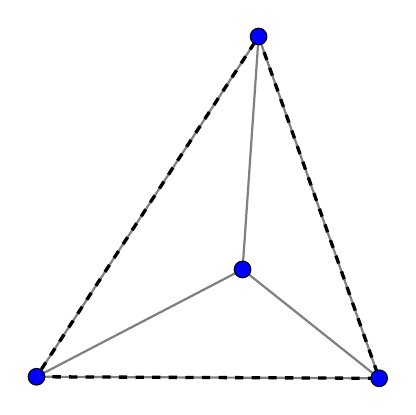
\begin{tikzpicture}[scale=1.5]
\newcommand{\x}{2}

  \draw [gray, thick] (0.423016, 4.503319) -- (2.303165, 7.383978);
  \draw [gray, thick] (0.423016, 4.503319) -- (3.32398, 4.490406);
  \draw [gray, thick] (0.423016, 4.503319) -- (2.167452, 5.411797);

  \draw [gray, thick] (3.32398, 4.490406) -- (2.303165, 7.383978);
  \draw [gray, thick] (2.167452, 5.411797) -- (3.32398, 4.490406);
  \draw [gray, thick] (2.303165, 7.383978) -- (2.167452, 5.411797);

  \draw[dashed, very thick]
    (2.30317, 7.38398)
     -- (3.32398, 4.490406)
     -- (0.42302, 4.503321)
     -- cycle;

\vertex{0.423016}{4.503319}{\x};
\vertex{2.303165}{7.383978}{\x};
\vertex{2.167452}{5.411797}{\x};
\vertex{3.32398}{4.490404}{\x};

\end{tikzpicture}
	
}

\frame{
	\frametitle{Upperbound for $4$-Hole: $h(4) = 5$}

\large

   \newcommand{\x}{0.75}


\centering
	
	
\begin{tikzpicture}[scale=2.5]

  \draw[shift={(1, 3.04)}, scale=1.5, thick]
    (0, 0)
     -- (0.64, 0.32)
     -- (1.12, 0)
     -- (0.8, -0.48)
     -- (0.32, -0.48)
     -- cycle;

\only<2->{
  \filldraw[shift={(1, 3.04)}, scale=1.5, draw=structure, very thick, fill=structure!30!white]
    (0, 0)
     -- (0.64, 0.32)
     -- (1.12, 0)
 %    -- (0.8, -0.48)
     -- (0.32, -0.48)
     -- cycle;     
}
     
  \vertex{2.2}{2.32}{\x};
  \vertex{2.68}{3.04}{\x};
  \vertex{1.96}{3.52}{\x};
  \vertex{1}{3.04}{\x};
  \vertex{1.48}{2.32}{\x};

\end{tikzpicture}
~~~~~~~~~~~~~~~~~~~~
\pause
\pause
\begin{tikzpicture}[scale=2.5]
  \draw[shift={(3.8, 2.32)}, scale=1.5, thick]
    (0, 0)
     -- (0, 0.8)
     -- (0.8, 0.64)
     -- (0.64, 0.16)
     -- cycle;

  \draw[shift={(3.8, 3.52)}, scale=1.5]
    (0, 0)
     -- (0.64, -0.64);
  \draw[shift={(3.8, 2.32)}, scale=1.5]
    (0, 0)
     -- (0.8, 0.64);

\only<4->{
  \filldraw[shift={(3.8, 3.52)}, scale=1.5, draw=structure, very thick, fill=structure!30!white]
    (0, 0)
     -- (0.16, -0.48)
     -- (0.64, -0.64)
     -- (0.8, -0.16)
     -- cycle;
     
   \draw[shift={(3.8, 3.52)}, scale=1.5]
    (0, 0)
     -- (0.64, -0.64);
  \draw[shift={(3.8, 2.32)}, scale=1.5]
    (0, 0)
     -- (0.8, 0.64);
}

  \vertex{4.04}{2.8}{\x};
  \vertex{3.8}{3.52}{\x};
  \vertex{5}{3.28}{\x};
  \vertex{4.76}{2.56}{\x};
  \vertex{3.8}{2.32}{\x};

\end{tikzpicture}

\pause
\pause
	
\begin{tikzpicture}[scale=2.5]
     
  
    \draw[shift={(5.72, 2.56)}, scale=1.5]
    (0, 0)
     -- (1.28, 0.48);

  \draw[shift={(5.96, 2.32)}, scale=1.5, thick]
    (0, 0)
     -- (0.48, 0.96)
     -- (0.96, 0.16)
     -- cycle;

\only<6->{

    \draw[shift={(5.72, 2.56)}, scale=1.5]
    (0, 0)
     -- (1.28, 0.48);
     
  \filldraw[shift={(5.96, 2.32)}, scale=1.5, draw=structure, very thick, fill=structure!30!white]
    (0, 0)
     -- (0.3426, 0.348475)
     -- (0.59104, 0.44164)
     -- (0.96, 0.16)
     -- cycle;
 }
 
  \vertex{6.4739}{2.842713}{\x};
  \vertex{6.84656}{2.98246}{\x};
  \vertex{5.96}{2.32}{\x};
  \vertex{6.68}{3.76}{\x};
  \vertex{7.4}{2.56}{\x};
  

  \end{tikzpicture}
	
}

\frame{
	\frametitle{Lowerbound for $5$-Hole: $h(5) \geq 10$}

\large

\begin{center}
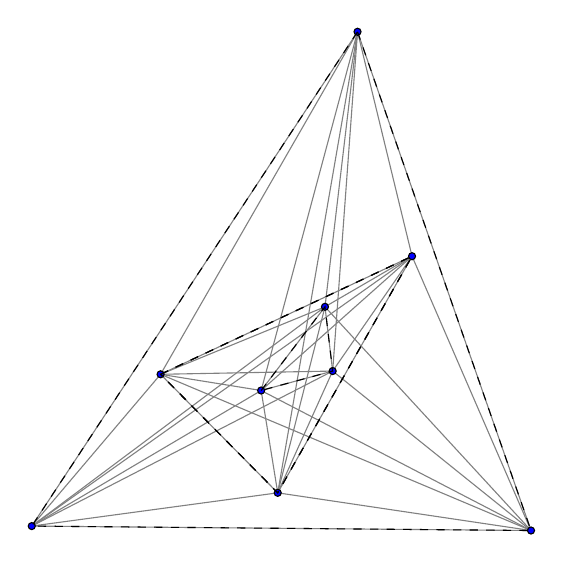
\begin{tikzpicture}[scale=1.7]
\newcommand{\x}{0.75}
\draw[shift={(1.26017, 1.37339)}, rotate=-89.8437, scale=0.63, gray]
  (0, 0)
   -- (-5.85132, 3.87897);
\draw[shift={(1.26017, 1.37339)}, rotate=-89.8437, scale=0.63, gray]
  (0, 0)
   -- (-3.18788, 4.5182);
\draw[shift={(1.26017, 1.37339)}, rotate=-89.8437, scale=0.63, gray]
  (0, 0)
   -- (-1.79574, 1.53246);
\draw[shift={(1.26017, 1.37339)}, rotate=-89.8437, scale=0.63, gray]
  (0, 0)
   -- (-2.59075, 3.48411);
\draw[shift={(1.26017, 1.37339)}, rotate=-89.8437, scale=0.63, gray]
  (0, 0)
   -- (-1.60036, 2.7245);
\draw[shift={(1.26017, 1.37339)}, rotate=-89.8437, scale=0.63, gray]
  (0, 0)
   -- (-1.82854, 3.57324);
\draw[shift={(1.26017, 1.37339)}, rotate=-89.8437, scale=0.63, gray]
  (0, 0)
   -- (-0.38641, 2.91774);
\draw[shift={(1.26017, 1.37339)}, rotate=-89.8437, scale=0.63, gray]
  (0, 0)
   -- (0.06868, 5.92);
\draw[shift={(3.69386, 5.06637)}, rotate=-89.8437, scale=0.63, gray]
  (0, 0)
   -- (2.66344, 0.63923);
\draw[shift={(3.69386, 5.06637)}, rotate=-89.8437, scale=0.63, gray]
  (0, 0)
   -- (4.05558, -2.34651);
\draw[shift={(3.69386, 5.06637)}, rotate=-89.8437, scale=0.63, gray]
  (0, 0)
   -- (3.26057, -0.39486);
\draw[shift={(3.69386, 5.06637)}, rotate=-89.8437, scale=0.63, gray]
  (0, 0)
   -- (4.25096, -1.15447);
\draw[shift={(3.69386, 5.06637)}, rotate=-89.8437, scale=0.63, gray]
  (0, 0)
   -- (4.02278, -0.30573);
\draw[shift={(3.69386, 5.06637)}, rotate=-89.8437, scale=0.63, gray]
  (0, 0)
   -- (5.46491, -0.96123);
\draw[shift={(3.69386, 5.06637)}, rotate=-89.8437, scale=0.63, gray]
  (0, 0)
   -- (5.92, 2.04103);
\draw[shift={(4.10115, 3.38951)}, rotate=-89.8437, scale=0.63, gray]
  (0, 0)
   -- (1.39214, -2.98574);
\draw[shift={(4.10115, 3.38951)}, rotate=-89.8437, scale=0.63, gray]
  (0, 0)
   -- (0.59713, -1.03409);
\draw[shift={(4.10115, 3.38951)}, rotate=-89.8437, scale=0.63, gray]
  (0, 0)
   -- (1.58752, -1.7937);
\draw[shift={(4.10115, 3.38951)}, rotate=-89.8437, scale=0.63, gray]
  (0, 0)
   -- (1.35934, -0.94496);
\draw[shift={(4.10115, 3.38951)}, rotate=-89.8437, scale=0.63, gray]
  (0, 0)
   -- (2.80147, -1.60046);
\draw[shift={(4.10115, 3.38951)}, rotate=-89.8437, scale=0.63, gray]
  (0, 0)
   -- (3.25656, 1.4018);
\draw[shift={(2.22253, 2.50734)}, rotate=-89.8437, scale=0.63, gray]
  (0, 0)
   -- (-0.79501, 1.95165);
\draw[shift={(2.22253, 2.50734)}, rotate=-89.8437, scale=0.63, gray]
  (0, 0)
   -- (0.19538, 1.19204);
\draw[shift={(2.22253, 2.50734)}, rotate=-89.8437, scale=0.63, gray]
  (0, 0)
   -- (-0.0328, 2.04078);
\draw[shift={(2.22253, 2.50734)}, rotate=-89.8437, scale=0.63, gray]
  (0, 0)
   -- (1.40933, 1.38528);
\draw[shift={(2.22253, 2.50734)}, rotate=-89.8437, scale=0.63, gray]
  (0, 0)
   -- (1.86442, 4.38754);
\draw[shift={(3.4507, 3.01154)}, rotate=-89.8437, scale=0.63, gray]
  (0, 0)
   -- (0.99039, -0.75961);
\draw[shift={(3.4507, 3.01154)}, rotate=-89.8437, scale=0.63, gray]
  (0, 0)
   -- (0.76221, 0.08913);
\draw[shift={(3.4507, 3.01154)}, rotate=-89.8437, scale=0.63, gray]
  (0, 0)
   -- (2.20434, -0.56637);
\draw[shift={(3.4507, 3.01154)}, rotate=-89.8437, scale=0.63, gray]
  (0, 0)
   -- (2.65943, 2.43589);
\draw[shift={(2.97385, 2.38629)}, rotate=-89.8437, scale=0.63, gray]
  (0, 0)
   -- (-0.22818, 0.84874);
\draw[shift={(2.97385, 2.38629)}, rotate=-89.8437, scale=0.63, gray]
  (0, 0)
   -- (1.21395, 0.19324);
\draw[shift={(2.97385, 2.38629)}, rotate=-89.8437, scale=0.63, gray]
  (0, 0)
   -- (1.66904, 3.1955);
\draw[shift={(3.50817, 2.53151)}, rotate=-89.8437, scale=0.63, gray]
  (0, 0)
   -- (1.44213, -0.6555);
\draw[shift={(3.50817, 2.53151)}, rotate=-89.8437, scale=0.63, gray]
  (0, 0)
   -- (1.89722, 2.34676);
\draw[shift={(3.09768, 1.62184)}, rotate=-89.8437, scale=0.63, gray]
  (0, 0)
   -- (0.45509, 3.00226);
\vertex{1.26017}{1.37339}{\x};
\vertex{3.69386}{5.06637}{\x};
\vertex{4.10115}{3.38951}{\x};
\vertex{2.22253}{2.50734}{\x};
\vertex{3.4507}{3.01154}{\x};
\vertex{2.97385}{2.38629}{\x};
\vertex{3.50817}{2.53151}{\x};
\vertex{3.09768}{1.62184}{\x};
\vertex{4.98988}{1.34029}{\x};
\draw[dashed]
  (3.69386, 5.06637)
   -- (4.98988, 1.34029)
   -- (1.26017, 1.37339)
   -- cycle;
\draw[dashed]
  (2.22254, 2.50733)
   -- (4.10115, 3.38951)
   -- (3.09768, 1.62184)
   -- cycle;
\draw[dashed]
  (2.22254, 2.50733)
   -- (4.10115, 3.38951)
   -- (3.09768, 1.62184)
   -- cycle;
\draw[dashed]
  (2.97385, 2.38629)
   -- (3.4507, 3.01154)
   -- (3.50817, 2.53151)
   -- cycle;
\end{tikzpicture}
\end{center}

All 5-gons in these 9 points have an inner point: $h(5) = 10$
	
}

\frame{
	\frametitle{Lowerbound for $6$-Hole: $h(6) \geq 30$}

\large

\begin{center}
	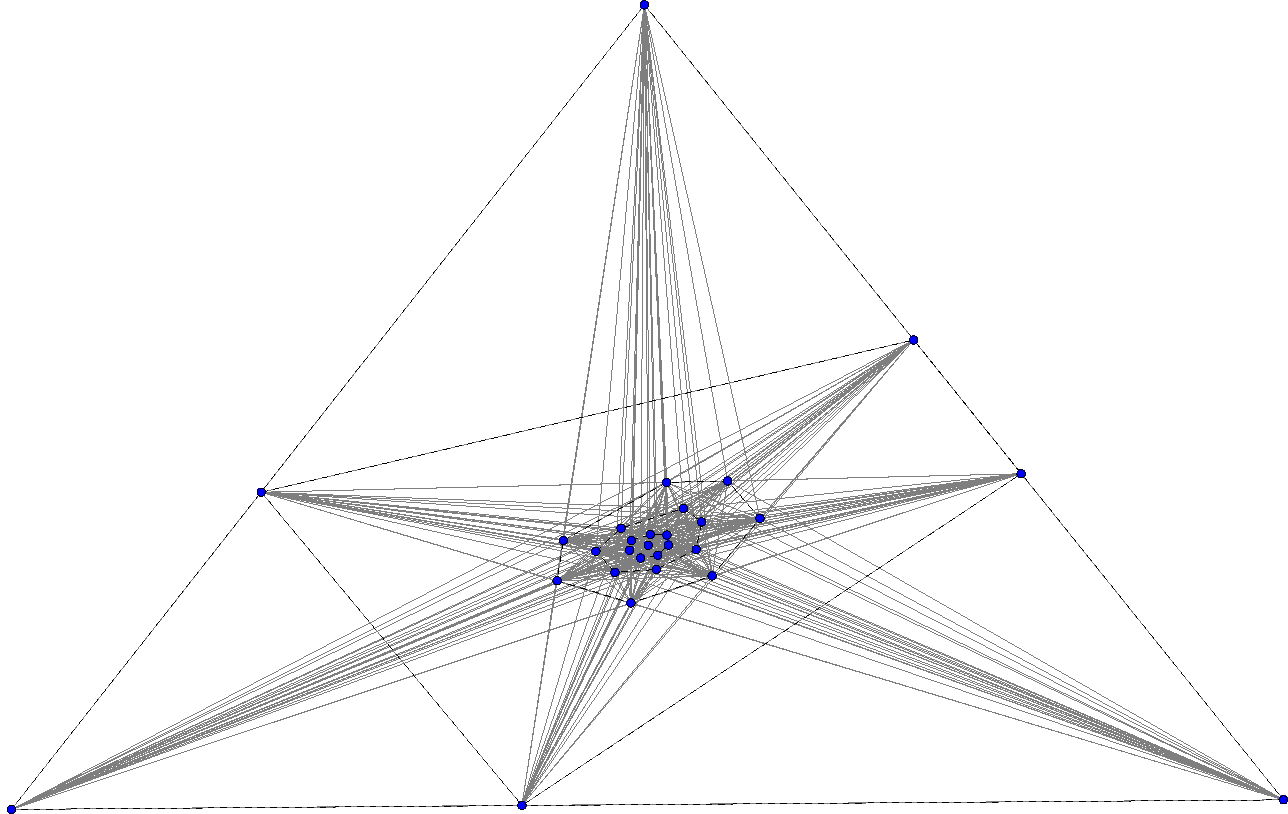
\includegraphics[width=.75\textwidth]{lb6hole.pdf}
\end{center}

29 points, no $6$-hole \textcolor{xgreen}{[Overmars ’02]}
\begin{itemize}
\item Found using simulated annealing... is now \structure{easy using SAT}
\item This contains $7$-gon. Each $9$-gon contains a $6$-hole
\end{itemize}

}

\frame{
	\frametitle{No Lowerbound for $7$-Hole: Horton's Construction (I)}


\bigskip
\bigskip

\begin{minipage}{.45\textwidth}
\centering

\begin{tikzpicture}[scale=1.5]

\node[draw,circle, fill=blue, scale=0.3] (a) at (2.786402,4.8952) {};
\node[draw,circle, fill=structure, scale=0.3] (b) at (0.6552,4.8952) {};


\draw[gray] (a) -- (b) ;


 
\end{tikzpicture}

\bigskip

$2^1$ points, no 7-hole

\bigskip
\bigskip
\bigskip

\pause

\begin{tikzpicture}[scale=1.5]

\node[draw,circle, fill=structure, scale=0.3] (a) at (2.786402,4.8952) {};
\node[draw,circle, fill=blue, scale=0.3] (c) at (3.852003,5.8276) {};
\node[draw,circle, fill=structure, scale=0.3] (b) at (0.6552,4.8952) {};
\node[draw,circle, fill=blue, scale=0.3] (d) at (1.720801,5.8276) {};


\draw[structure, thick] (a) -- (b) ;
\draw[gray] (a) -- (c) (a) -- (d) (b) -- (c) (b) -- (d) ; 
\draw[blue, thick] (c) -- (d); 

 
\end{tikzpicture}

\bigskip

$2^2$ points, no 7-hole

\end{minipage}
~~~\pause
\begin{minipage}{.45\textwidth}
\centering
\begin{tikzpicture}[scale=1.5]

\node[draw,circle, fill=structure, scale=0.3] (a) at (2.786402,4.8952) {};
\node[draw,circle, fill=structure, scale=0.3] (b) at (3.852003,5.8276) {};
\node[draw,circle, fill=structure, scale=0.3] (c) at (0.6552,4.8952) {};
\node[draw,circle, fill=structure, scale=0.3] (d) at (1.720801,5.8276) {};

\node[draw,circle, fill=blue, scale=0.3] (e) at (1.188,7.6924) {};
\node[draw,circle, fill=blue, scale=0.3] (f) at (3.319199,7.6924) {};
\node[draw,circle, fill=blue, scale=0.3] (g) at (2.253598,8.6248) {};
\node[draw,circle, fill=blue, scale=0.3] (h) at (4.3848,8.6248) {};

\draw[structure, thick] (a) -- (b) (a) -- (c) (a) -- (d) (c) -- (d) (b) -- (c) (b) -- (d);
\draw[gray]  (a) -- (e) (a) -- (f) (a) -- (g) (a) -- (h) (b) -- (e) (b) -- (f) (b) -- (g) (b) -- (h);
\draw[gray] (c) -- (d)  (c) -- (e) (c) -- (f) (c) -- (g) (c) -- (h);
\draw[gray] (d) -- (e) (d) -- (f) (d) -- (g) (d) -- (h);
\draw[blue, thick] (e) -- (f) (e) -- (g) (e) -- (h);
\draw[blue, thick] (f) -- (g) (f) -- (h)  (g) -- (h);


 
\end{tikzpicture}

\bigskip

$2^3$ points, no 7-hole
\end{minipage}
	
}

\frame{
	\frametitle{No Lowerbound for $7$-Hole: Horton's Construction (II)}

\centering

\begin{tikzpicture}[scale=1.7]

\node[draw,circle, fill=structure, scale=0.3] (a) at (0.6552, 5.1752) {};
\node[draw,circle, fill=structure, scale=0.3] (b) at (2.644318, 5.1752) {};
\node[draw,circle, fill=structure, scale=0.3] (c) at (1.649762, 5.29175) {};
\node[draw,circle, fill=structure, scale=0.3] (d) at (3.63888, 5.29175) {};
\node[draw,circle, fill=structure, scale=0.3] (e) at (1.15248, 5.52485) {};
\node[draw,circle, fill=structure, scale=0.3] (f) at (3.141602, 5.52485) {};
\node[draw,circle, fill=structure, scale=0.3] (g) at (2.14704, 5.6414) {};
\node[draw,circle, fill=structure, scale=0.3] (h) at (4.136158, 5.6414) {};
\node[draw,circle, fill=blue, scale=0.3] (i) at (0.90384, 8.4386) {};
\node[draw,circle, fill=blue, scale=0.3] (j) at (2.89296, 8.4386) {};
\node[draw,circle, fill=blue, scale=0.3] (k) at (1.898398, 8.55515) {};
\node[draw,circle, fill=blue, scale=0.3] (l) at (3.887522, 8.55515) {};
\node[draw,circle, fill=blue, scale=0.3] (m) at (1.40112, 8.78825) {};
\node[draw,circle, fill=blue, scale=0.3] (n) at (3.390238, 8.78825) {};
\node[draw,circle, fill=blue, scale=0.3] (o) at (2.395682, 8.9048) {};
\node[draw,circle, fill=blue, scale=0.3] (p) at (4.3848, 8.9048) {};
 
 
\draw[structure,thick] (a) -- (b) (a) -- (c) (a) -- (d) (a) -- (e) (a) -- (f) (a) -- (g) (a) -- (h);
\draw[structure,thick] (b) -- (c) (b) -- (d) (b) -- (e) (b) -- (f) (b) -- (g) (b) -- (h);
\draw[structure,thick] (c) -- (d) (c) -- (e) (c) -- (f) (c) -- (g) (c) -- (h);
\draw[structure,thick] (d) -- (e) (d) -- (f) (d) -- (g) (d) -- (h); 
\draw[structure,thick] (e) -- (f) (e) -- (g) (e) -- (h) ;
\draw[structure,thick] (f) -- (g) (f) -- (h) ;
\draw[structure,thick] (g) -- (h) ;
\draw[gray] (a) -- (i) (a) -- (j) (a) -- (k) (a) -- (l) (a) -- (m) (a) -- (n) (a) -- (o) (a) -- (p);
\draw[gray] (b) -- (i) (b) -- (j) (b) -- (k) (b) -- (l) (b) -- (m) (b) -- (n) (b) -- (o) (b) -- (p);
\draw[gray] (c) -- (i) (c) -- (j) (c) -- (k) (c) -- (l) (c) -- (m) (c) -- (n) (c) -- (o) (c) -- (p);
\draw[gray] (d) -- (i) (d) -- (j) (d) -- (k) (d) -- (l) (d) -- (m) (d) -- (n) (d) -- (o) (d) -- (p);
\draw[gray] (e) -- (i) (e) -- (j) (e) -- (k) (e) -- (l) (e) -- (m) (e) -- (n) (e) -- (o) (e) -- (p);
\draw[gray] (f) -- (i) (f) -- (j) (f) -- (k) (f) -- (l) (f) -- (m) (f) -- (n) (f) -- (o) (f) -- (p);
\draw[gray] (g) -- (i) (g) -- (j) (g) -- (k) (g) -- (l) (g) -- (m) (g) -- (n) (g) -- (o) (g) -- (p);
 \draw[gray] (h) -- (i) (h) -- (j) (h) -- (k) (h) -- (l) (h) -- (m) (h) -- (n) (h) -- (o) (h) -- (p);
\draw[blue,thick] (i) -- (j) (i) -- (k) (i) -- (l) (i) -- (m) (i) -- (n) (i) -- (o) (i) -- (p);
\draw[blue,thick] (j) -- (k) (j) -- (l) (j) -- (m) (j) -- (n) (j) -- (o) (j) -- (p);
\draw[blue,thick] (k) -- (l) (k) -- (m) (k) -- (n) (k) -- (o) (k) -- (p);
\draw[blue,thick] (l) -- (m) (l) -- (n) (l) -- (o) (l) -- (p);
\draw[blue,thick] (m) -- (n) (m) -- (o) (m) -- (p);
\draw[blue,thick] (n) -- (o) (n) -- (p) (o) -- (p);
 
 \node[draw,circle, fill=structure, scale=0.3] (a) at (0.6552, 5.1752) {};
\node[draw,circle, fill=structure, scale=0.3] (b) at (2.644318, 5.1752) {};
\node[draw,circle, fill=structure, scale=0.3] (c) at (1.649762, 5.29175) {};
\node[draw,circle, fill=structure, scale=0.3] (d) at (3.63888, 5.29175) {};
\node[draw,circle, fill=structure, scale=0.3] (e) at (1.15248, 5.52485) {};
\node[draw,circle, fill=structure, scale=0.3] (f) at (3.141602, 5.52485) {};
\node[draw,circle, fill=structure, scale=0.3] (g) at (2.14704, 5.6414) {};
\node[draw,circle, fill=structure, scale=0.3] (h) at (4.136158, 5.6414) {};
\node[draw,circle, fill=blue, scale=0.3] (i) at (0.90384, 8.4386) {};
\node[draw,circle, fill=blue, scale=0.3] (j) at (2.89296, 8.4386) {};
\node[draw,circle, fill=blue, scale=0.3] (k) at (1.898398, 8.55515) {};
\node[draw,circle, fill=blue, scale=0.3] (l) at (3.887522, 8.55515) {};
\node[draw,circle, fill=blue, scale=0.3] (m) at (1.40112, 8.78825) {};
\node[draw,circle, fill=blue, scale=0.3] (n) at (3.390238, 8.78825) {};
\node[draw,circle, fill=blue, scale=0.3] (o) at (2.395682, 8.9048) {};
\node[draw,circle, fill=blue, scale=0.3] (p) at (4.3848, 8.9048) {};
 
  
\end{tikzpicture}

\bigskip

 $2^4$ points, no 7-hole


}

\frame{
	\frametitle{No Lowerbound for $7$-Hole: Horton's Construction (III)}
	
	\centering
	
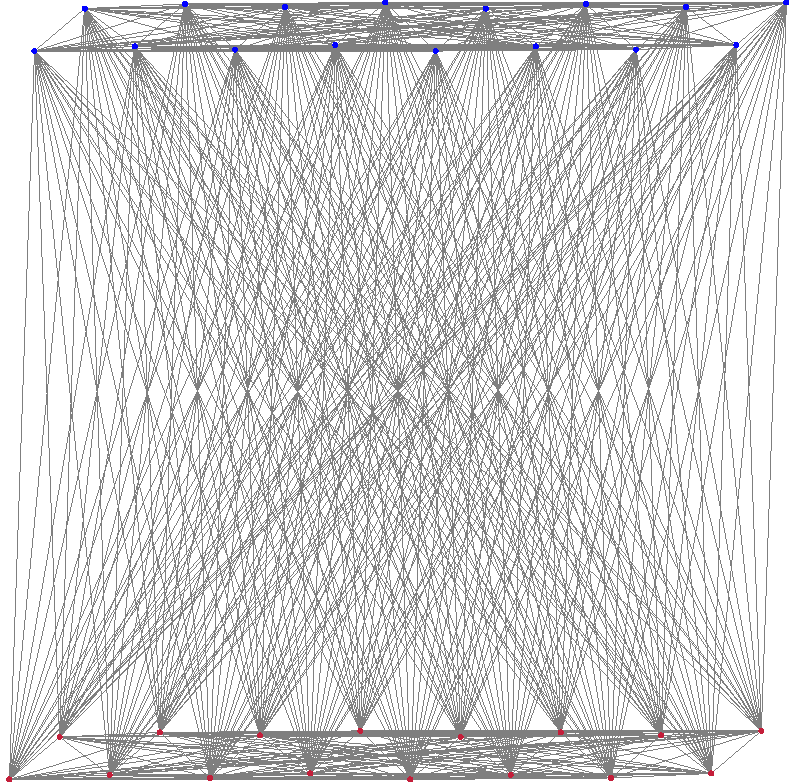
\includegraphics[height=180pt]{7hole-final.pdf}
	
	\bigskip
	
	 $2^5$ points, no 7-hole

}


\section{SAT Encoding}
\frame{\Large \tableofcontents[currentsection]}


\frame{
	\frametitle{Orientation Variables}
	
\large 
\begin{minipage}{.62\textwidth}

No explicit \structure{coordinates} of points

\bigskip

Instead for every triple $a < b < c$,\\ one \structure{orientation variable  $O_{a,b,c}$}
to denote whether point $c$ is above the line $ab$

\bigskip

Not all assignments are \structure{realizable}
\begin{itemize}
\item Realizability is a notoriously hard problem
\textcolor{xgreen}{[Mnëv '88]}
\end{itemize}

\bigskip

\structure{Axioms} (next slide) eliminate many\\
unrealizable assignments

\bigskip

\end{minipage}	
\begin{minipage}{.35\textwidth}
\centering
\begin{tikzpicture}
\newcommand{\x}{2}
\node (a) at (2.72, 6.48) {~};
\node (b) at (4.48, 6.24) {~};
\node (c) at (4.72, 7.12) {~};
\node (d) at (4.8, 3.36) {~};

  \draw[shift={(2.24083, 6.54534)}, scale=2]
    (0, 0)
     -- (1.76, -0.24);
  \draw[xgreen, thick, ->]
    (3.2, 6.55)
     .. controls (4.25, 6.35) and (4.4, 6.5) .. (4.5, 6.85);
  \draw[structure, thick, ->]
    (3, 6.2)
     .. controls (4.25, 5.9) and (4.4, 5.8) .. (4.5, 4.4);

%  \draw[shift={(2.8754, 6.36479)}, scale=1, red, very thick, ->]
%    (0, 0)
%     .. controls (1.584, -0.216) and (1.52, -0.4) .. (0.48, -0.72);
  \node[font=\large, text=xgreen]
     at (3.9, 6.65) {+};
  \node[font=\large, text=structure]
     at (3.75, 5.5) {--};
  \node 
     at (2.45, 6.7) {$a$};
  \node
     at (4.74, 6.42) {$b$};
  \node[text=xgreen]
     at (4.85, 7.35) {$c$};
  \node[text=structure]
     at (4.88, 3.12) {$d$};
  \draw[gray]
    (b)
     -- (c)
     -- (a);
  \draw[gray]
    (b)
     -- (d)
     -- (a);
     
\vertex{2.72}{6.48}{\x};
\vertexc{4.8}{3.36}{\x}{structure}; 
\vertex{(4.48}{6.24}{\x};
\vertexc{4.72}{7.12}{\x}{xgreen};
%  \node
%     at (5.07475, 6.26071) {$e$};
%\vertex{0.0491475}{0.0618071}{\x};
\end{tikzpicture}
\end{minipage}
	
}

\frame{
	\frametitle{Axioms}

\large

$\forall a < b < c < d$: ``at most one sign change''


\begin{center}
\begin{minipage}{.5\textwidth}
\begin{tikzpicture}[scale=1.3]
\newcommand{\x}{1.5}
\vertex{.32}{6.56}{\x};
\vertex{1.12}{6.24}{\x};
\vertex{1.92}{6.72}{\x};
  \draw[shift={(.32, 6.56)}, scale=3.414]
    (0, 0)
     -- (.80, -.32);
  \draw[shift={(1.12, 6.24001)}, scale=2.5322]
    (0, 0)
     -- (.80, .48);
  \draw[shift={(3.5081, 6.8788)}, scale=1.9926]
    (0, 0)
     -- (-1.60, -.16);
\only<4->{
\vertexc{2.72}{5.12}{\x}{xorange};}
\only<3->{
\vertexc{2.72}{6.24}{\x}{cyan};}
\only<2->{
\vertexc{2.72}{7.04}{\x}{xgreen};}
\vertexc{2.72}{7.68}{\x}{structure};
  \node
     at (.16, 6.24) {$a$};
  \node
     at (.96, 5.92) {$b$};
  \node
     at (1.76, 6.88) {$c$};
  \node
     at (2.72, 8.5) {$d$};
  \node
     at (2.72, 5) {$~$};
\end{tikzpicture}

\end{minipage}
\begin{minipage}{.4\textwidth}


\begin{tabular}{cccc}
\toprule
$O_{abc}$ & $O_{abd}$ & $O{acd}$ & $O_{bcd}$\\
\midrule
\textcolor{structure}{$+$} & \textcolor{structure}{$+$} & \textcolor{structure}{$+$} & \textcolor{structure}{$+$}\\
\pause
\textcolor{xgreen}{$+$} & \textcolor{xgreen}{$+$} & \textcolor{xgreen}{$+$} & \textcolor{xgreen}{$-$}\\
\pause
\textcolor{cyan}{$+$} & \textcolor{cyan}{$+$} & \textcolor{cyan}{$-$} & \textcolor{cyan}{$-$}\\
\pause
\textcolor{xorange}{$+$} & \textcolor{xorange}{$-$} & \textcolor{xorange}{$-$} & \textcolor{xorange}{$-$}\\
\pause
$-$ & $-$ & $-$ & $-$\\
$-$ & $-$ & $-$ & $+$\\
$-$ & $-$ & $+$ & $+$\\
$-$ & $+$ & $+$ & $+$\\
\bottomrule
\end{tabular}

\end{minipage}
\end{center}

Block multiple sign changes with $\Theta(n^4)$ (ternary) clauses \textcolor{xgreen}{[Felsner \& Weil ’01]}


}

\frame{
	\frametitle{$k$-Gon Encoding: Forbidding a $k$-Gon}

\large

\begin{minipage}{.47\textwidth}
\centering
$O_{a,b,c} \lor O_{b,c,d} \lor O_{c,d,e} \lor O_{d,e,f}$
\end{minipage}
\hfill
\begin{minipage}{.47\textwidth}
\centering
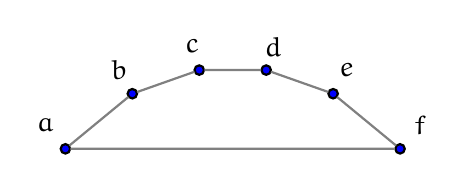
\begin{tikzpicture}[xscale=0.85]
\node at (-0.3,0.3) {$a$};
\node at (0.8,1) {$b$};
\node at (1.9,1.3) {$c$};
\node at (3.1,1.3) {$d$};
\node at (4.2,1) {$e$};
\node at (5.3,0.3) {$f$};
\node[draw,circle, thick, fill=blue, scale=0.3] (a) at (0,0) {};
\node[draw,circle, thick, fill=blue, scale=0.3] (b) at (1,0.7) {};
\node[draw,circle, thick, fill=blue, scale=0.3] (c) at (2,1) {};
\node[draw,circle, thick, fill=blue, scale=0.3] (d) at (3,1) {};
\node[draw,circle, thick, fill=blue, scale=0.3] (e) at (4,0.7) {};
\node[draw,circle, thick, fill=blue, scale=0.3] (f) at (5,0) {};
\draw[gray, thick] (a) -- (b) -- (c) -- (d) -- (e) -- (f) -- (a);
%\draw[gray] (a) -- (b) -- (c) -- (a);
%\draw[gray] (a) -- (c) -- (d) -- (a);
%\draw[gray] (a) -- (d) -- (e) -- (a);
%\draw[gray] (a) -- (e) -- (f) -- (a);
\end{tikzpicture}
\end{minipage}

\begin{minipage}{.47\textwidth}
\centering
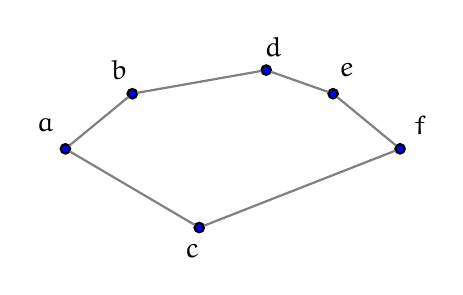
\begin{tikzpicture}[xscale=0.85]
\node at (-0.3,0.3) {$a$};
\node at (0.8,1) {$b$};
\node at (1.9,-1.3) {$c$};
\node at (3.1,1.3) {$d$};
\node at (4.2,1) {$e$};
\node at (5.3,0.3) {$f$};
\node[draw,circle, thick, fill=blue, scale=0.3] (a) at (0,0) {};
\node[draw,circle, thick, fill=blue, scale=0.3] (b) at (1,0.7) {};
\node[draw,circle, thick, fill=blue, scale=0.3] (c) at (2,-1) {};
\node[draw,circle, thick, fill=blue, scale=0.3] (d) at (3,1) {};
\node[draw,circle, thick, fill=blue, scale=0.3] (e) at (4,0.7) {};
\node[draw,circle, thick, fill=blue, scale=0.3] (f) at (5,0) {};
\draw[gray, thick] (a) -- (b) -- (d) -- (e) -- (f) -- (c) -- (a);
%\draw[gray] (a) -- (b) -- (d) -- (a);
%\draw[gray] (a) -- (c) -- (f) -- (a);
%\draw[gray] (a) -- (d) -- (e) -- (a);
%\draw[gray] (a) -- (e) -- (f) -- (a);
\end{tikzpicture}
\end{minipage}
\hfill
\begin{minipage}{.47\textwidth}
$O_{a,b,d} \lor O_{b,d,e} \lor O_{d,e,f} \lor \overline{O_{a,c,f}}$
\end{minipage}


\vspace{-10pt}

\begin{minipage}{.47\textwidth}
$O_{a,b,d} \lor O_{b,d,f} \lor \overline{O_{a,c,e}} \lor \overline{O_{c,e,f}}$
\end{minipage}
\hfill
\begin{minipage}{.47\textwidth}
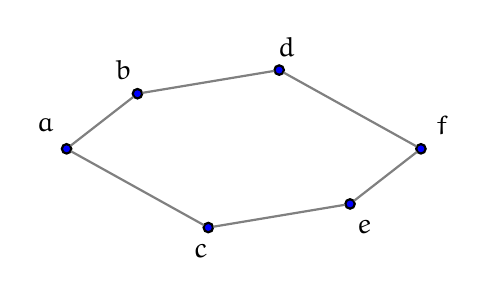
\begin{tikzpicture}[xscale=0.9]
\node at (-0.3,0.3) {$a$};
\node at (0.8,1) {$b$};
\node at (1.9,-1.3) {$c$};
\node at (3.1,1.3) {$d$};
\node at (4.2,-1) {$e$};
\node at (5.3,0.3) {$f$};
\node[draw,circle, thick, fill=blue, scale=0.3] (a) at (0,0) {};
\node[draw,circle, thick, fill=blue, scale=0.3] (b) at (1,0.7) {};
\node[draw,circle, thick, fill=blue, scale=0.3] (c) at (2,-1) {};
\node[draw,circle, thick, fill=blue, scale=0.3] (d) at (3,1) {};
\node[draw,circle, thick, fill=blue, scale=0.3] (e) at (4,-0.7) {};
\node[draw,circle, thick, fill=blue, scale=0.3] (f) at (5,0) {};
\draw[gray, thick] (a) -- (b) -- (d) -- (f) -- (e) -- (c) -- (a);
%\draw[gray] (a) -- (b) -- (d) -- (a);
%\draw[gray] (a) -- (c) -- (e) -- (a);
%\draw[gray] (a) -- (e) -- (f) -- (a);
%\draw[gray] (a) -- (d) -- (f) -- (a);
\end{tikzpicture}
\end{minipage}
}


\frame{
	\frametitle{Optimized $k$-Gon Encoding}

\large

\begin{minipage}{.47\textwidth}
%\centering
$x_{c,d} \lor O_{a,b,c} \lor O_{b,c,d}$\\
$\overline {x_{c,d}} \lor O_{c,d,e} \lor O_{d,e,f}$
\end{minipage}
\hfill
\begin{minipage}{.47\textwidth}
\centering
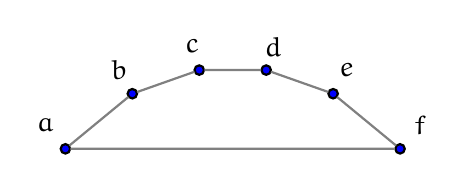
\begin{tikzpicture}[xscale=0.85]
\node at (-0.3,0.3) {$a$};
\node at (0.8,1) {$b$};
\node at (1.9,1.3) {$c$};
\node at (3.1,1.3) {$d$};
\node at (4.2,1) {$e$};
\node at (5.3,0.3) {$f$};
\node[draw,circle, thick, fill=blue, scale=0.3] (a) at (0,0) {};
\node[draw,circle, thick, fill=blue, scale=0.3] (b) at (1,0.7) {};
\node[draw,circle, thick, fill=blue, scale=0.3] (c) at (2,1) {};
\node[draw,circle, thick, fill=blue, scale=0.3] (d) at (3,1) {};
\node[draw,circle, thick, fill=blue, scale=0.3] (e) at (4,0.7) {};
\node[draw,circle, thick, fill=blue, scale=0.3] (f) at (5,0) {};
\draw[gray, thick] (a) -- (b) -- (c) -- (d) -- (e) -- (f) -- (a);
%\draw[gray] (a) -- (b) -- (c) -- (a);
%\draw[gray] (a) -- (c) -- (d) -- (a);
%\draw[gray] (a) -- (d) -- (e) -- (a);
%\draw[gray] (a) -- (e) -- (f) -- (a);
\end{tikzpicture}
\end{minipage}

\begin{minipage}{.47\textwidth}
\centering
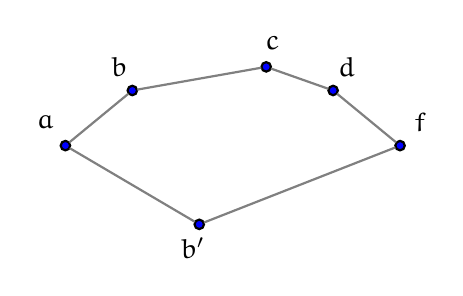
\begin{tikzpicture}[xscale=0.85]
\node at (-0.3,0.3) {$a$};
\node at (0.8,1) {$b$};
\node at (1.9,-1.3) {$b^{\prime}$};
\node at (3.1,1.3) {$c$};
\node at (4.2,1) {$d$};
\node at (5.3,0.3) {$f$};
\node[draw,circle, thick, fill=blue, scale=0.3] (a) at (0,0) {};
\node[draw,circle, thick, fill=blue, scale=0.3] (b) at (1,0.7) {};
\node[draw,circle, thick, fill=blue, scale=0.3] (c) at (2,-1) {};
\node[draw,circle, thick, fill=blue, scale=0.3] (d) at (3,1) {};
\node[draw,circle, thick, fill=blue, scale=0.3] (e) at (4,0.7) {};
\node[draw,circle, thick, fill=blue, scale=0.3] (f) at (5,0) {};
\draw[gray, thick] (a) -- (b) -- (d) -- (e) -- (f) -- (c) -- (a);
%\draw[gray] (a) -- (b) -- (d) -- (a);
%\draw[gray] (a) -- (c) -- (f) -- (a);
%\draw[gray] (a) -- (d) -- (e) -- (a);
%\draw[gray] (a) -- (e) -- (f) -- (a);
\end{tikzpicture}
\end{minipage}
\hfill
\begin{minipage}{.47\textwidth}
%\centering
$y_{a,f} \lor O_{a,b,c} \lor O_{b,c,d} \lor O_{c,d,f}$
$\overline{y_{a,f}} \lor \overline{O_{a,b^{\prime},f}}$

\end{minipage}


\vspace{-10pt}

\begin{minipage}{.47\textwidth}
%\centering
$z_{a,f} \lor O_{a,b,c} \lor O_{b,c,f}$\\
$\overline{z_{a,f}} \lor \overline{O_{a,b^{\prime},c^{\prime}}} \lor \overline{O_{b^{\prime},c^{\prime},f}}$\end{minipage}
\hfill
\begin{minipage}{.47\textwidth}
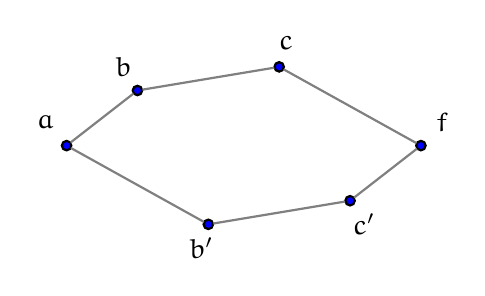
\begin{tikzpicture}[xscale=0.9]
\node at (-0.3,0.3) {$a$};
\node at (0.8,1) {$b$};
\node at (1.9,-1.3) {$b^{\prime}$};
\node at (3.1,1.3) {$c$};
\node at (4.2,-1) {$c^{\prime}$};
\node at (5.3,0.3) {$f$};
\node[draw,circle, thick, fill=blue, scale=0.3] (a) at (0,0) {};
\node[draw,circle, thick, fill=blue, scale=0.3] (b) at (1,0.7) {};
\node[draw,circle, thick, fill=blue, scale=0.3] (c) at (2,-1) {};
\node[draw,circle, thick, fill=blue, scale=0.3] (d) at (3,1) {};
\node[draw,circle, thick, fill=blue, scale=0.3] (e) at (4,-0.7) {};
\node[draw,circle, thick, fill=blue, scale=0.3] (f) at (5,0) {};
\draw[gray, thick] (a) -- (b) -- (d) -- (f) -- (e) -- (c) -- (a);
%\draw[gray] (a) -- (b) -- (d) -- (a);
%\draw[gray] (a) -- (c) -- (e) -- (a);
%\draw[gray] (a) -- (e) -- (f) -- (a);
%\draw[gray] (a) -- (d) -- (f) -- (a);
\end{tikzpicture}
\end{minipage}
}

\frame{
	\frametitle{Inside Variables}

\large

We introduce \structure{inside variables} $I_{x;a,b,c}$ which are true
if and only if point $x$ is in the triangle $abc$ with $a < x < b$
or $b < x < c$.

\bigskip

\begin{minipage}{.6\textwidth}
${I_{x;a,b,c}} \lor \overline{O_{a,b,c}} \lor {O_{a,x,b}} \lor \overline{O_{x,b,c}} \lor \overline{O_{a,x,c}}$\\[3pt]
$\overline{I_{x;a,b,c}} \lor \overline{O_{a,b,c}} \lor \overline{O_{a,x,b}}$\\[3pt]
$\overline{I_{x;a,b,c}} \lor \overline{O_{a,b,c}} \lor O_{x,b,c}$\\[3pt]
$\overline{I_{x;a,b,c}} \lor \overline{O_{a,b,c}} \lor O_{a,x,c}$\\[3pt]
\end{minipage}
%\hfill
\begin{minipage}{.35\textwidth}
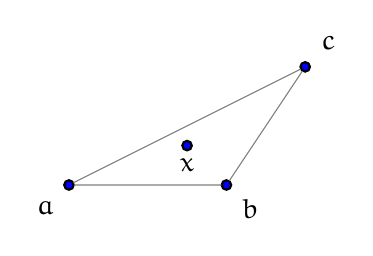
\begin{tikzpicture}

\node at (-0.3,-0.3) {$a$};
\node at (2.3,-0.3) {$b$};
\node at (3.3,1.8) {$c$};
\node at (1.5,0.25) {$x$};
\node[draw,circle, thick, fill=blue, scale=0.3] (a) at (0,0) {};
\node[draw,circle, thick, fill=blue, scale=0.3] (b) at (2,0) {};
\node[draw,circle, thick, fill=blue, scale=0.3] (c) at (3,1.5) {};
\node[draw,circle, thick, fill=blue, scale=0.3] (x) at (1.5,0.5) {};
\draw[gray] (a) -- (b) -- (c) -- (a);
\end{tikzpicture}
\end{minipage}

\pause
\bigskip

\begin{minipage}{.6\textwidth}

${I_{x;a,b,c}} \lor {O_{a,b,c}} \lor \overline{O_{a,x,b}} \lor O_{x,b,c} \lor O_{a,x,c}$\\[3pt]
$\overline{I_{x;a,b,c}} \lor {O_{a,b,c}} \lor {O_{a,x,b}}$\\[3pt]
$\overline{I_{x;a,b,c}} \lor {O_{a,b,c}} \lor \overline{O_{x,b,c}}$\\[3pt]
$\overline{I_{x;a,b,c}} \lor {O_{a,b,c}} \lor \overline{O_{a,x,c}}$\\[3pt]
\end{minipage}
\begin{minipage}{.35\textwidth}
\bigskip
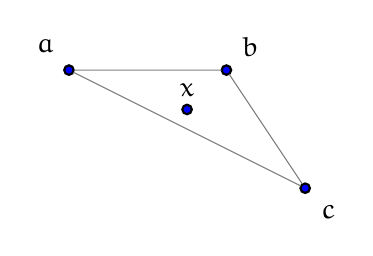
\begin{tikzpicture}

\node at (-0.3,0.3) {$a$};
\node at (2.3,0.3) {$b$};
\node at (3.3,-1.8) {$c$};
\node at (1.5,-0.25) {$x$};
\node[draw,circle, thick, fill=blue, scale=0.3] (a) at (0,0) {};
\node[draw,circle, thick, fill=blue, scale=0.3] (b) at (2,0) {};
\node[draw,circle, thick, fill=blue, scale=0.3] (c) at (3,-1.5) {};
\node[draw,circle, thick, fill=blue, scale=0.3] (x) at (1.5,-0.5) {};
\draw[gray] (a) -- (b) -- (c) -- (a);
\end{tikzpicture}
\end{minipage}

%  printf ("%i %i %i 0\n", -d,  t, -abx);
%  printf ("%i %i %i 0\n", -d,  t, -bcx);
%  printf ("%i %i %i 0\n", -d,  t, -acx);
%
%  printf ("%i %i %i 0\n", -d, -t,  abx);
%  printf ("%i %i %i 0\n", -d, -t,  bcx);
%  printf ("%i %i %i 0\n", -d, -t,  acx);
%
%#ifdef BLOCKED
%  printf ("%i %i %i %i %i 0\n", d,  t,  abx,  bcx,  acx);
%  printf ("%i %i %i %i %i 0\n", d, -t, -abx, -bcx, -acx);
%#endif

}

\frame{
	\frametitle{Hole Variables}
	
\large

We introduce \structure{hole variables} $H_{a,b,c}$ which are true
if and only if no points occur with the triangle $abc$ with $a < b < c$.

\medskip

\[
H_{a,b,c} \lor \bigvee_{a < x < c} {I_{x;a,b,c}}
\]

\[
\bigwedge_{a < x < c} \overline{H_{a,b,c}} \lor \overline{I_{x;a,b,c}}~~~~~~~\mathrm{(redundant)}
\]

\bigskip
\pause

Simple $6$-hole encoding:

\begin{center}
$(\bigvee_{a,b,c \in X} \overline H_{a,b,c})$~~~~$\forall~X \subset S$ with $|X| = 6$
\end{center}

}

\frame{
	\frametitle{$k$-Hole Encoding}

\large

\bigskip

\begin{minipage}{.52\textwidth}
%\centering
$O_{a,b,c} \lor O_{b,c,d} \lor O_{c,d,e} \lor O_{d,e,f}~\lor$\\[3pt]
$\overline{H_{a,b,c}} \lor \overline{H_{a,c,d}} \lor \overline{H_{a,d,e}} \lor \overline{H_{a,e,f}}$\\
\end{minipage}
\hfill
\begin{minipage}{.45\textwidth}
\centering
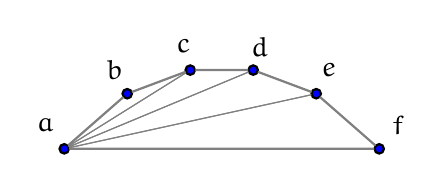
\begin{tikzpicture}[xscale=0.8]
\node at (-0.3,0.3) {$a$};
\node at (0.8,1) {$b$};
\node at (1.9,1.3) {$c$};
\node at (3.1,1.3) {$d$};
\node at (4.2,1) {$e$};
\node at (5.3,0.3) {$f$};
\node[draw,circle, thick, fill=blue, scale=0.3] (a) at (0,0) {};
\node[draw,circle, thick, fill=blue, scale=0.3] (b) at (1,0.7) {};
\node[draw,circle, thick, fill=blue, scale=0.3] (c) at (2,1) {};
\node[draw,circle, thick, fill=blue, scale=0.3] (d) at (3,1) {};
\node[draw,circle, thick, fill=blue, scale=0.3] (e) at (4,0.7) {};
\node[draw,circle, thick, fill=blue, scale=0.3] (f) at (5,0) {};
\draw[gray, thick] (a) -- (b) -- (c) -- (d) -- (e) -- (f) -- (a);
\draw[gray] (a) -- (b) -- (c) -- (a);
\draw[gray] (a) -- (c) -- (d) -- (a);
\draw[gray] (a) -- (d) -- (e) -- (a);
\draw[gray] (a) -- (e) -- (f) -- (a);
\end{tikzpicture}
\end{minipage}

\begin{minipage}{.45\textwidth}
\centering
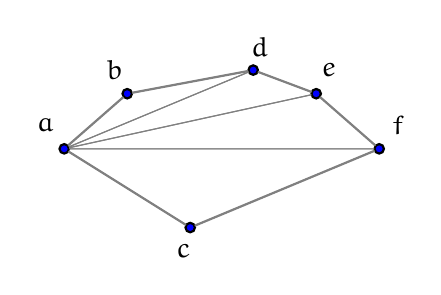
\begin{tikzpicture}[xscale=0.8]
\node at (-0.3,0.3) {$a$};
\node at (0.8,1) {$b$};
\node at (1.9,-1.3) {$c$};
\node at (3.1,1.3) {$d$};
\node at (4.2,1) {$e$};
\node at (5.3,0.3) {$f$};
\node[draw,circle, thick, fill=blue, scale=0.3] (a) at (0,0) {};
\node[draw,circle, thick, fill=blue, scale=0.3] (b) at (1,0.7) {};
\node[draw,circle, thick, fill=blue, scale=0.3] (c) at (2,-1) {};
\node[draw,circle, thick, fill=blue, scale=0.3] (d) at (3,1) {};
\node[draw,circle, thick, fill=blue, scale=0.3] (e) at (4,0.7) {};
\node[draw,circle, thick, fill=blue, scale=0.3] (f) at (5,0) {};
\draw[gray, thick] (a) -- (b) -- (d) -- (e) -- (f) -- (c) -- (a);
\draw[gray] (a) -- (b) -- (d) -- (a);
\draw[gray] (a) -- (c) -- (f) -- (a);
\draw[gray] (a) -- (d) -- (e) -- (a);
\draw[gray] (a) -- (e) -- (f) -- (a);
\end{tikzpicture}
\end{minipage}
\hfill
\begin{minipage}{.52\textwidth}
$O_{a,b,d} \lor O_{b,d,e} \lor O_{d,e,f} \lor \overline{O_{a,c,f}}~\lor$\\[3pt]
$\overline{H_{a,b,d}} \lor \overline{H_{a,d,e}} \lor \overline{H_{a,e,f}} \lor \overline{H_{a,c,f}}$
\end{minipage}


\vspace{-10pt}

\begin{minipage}{.52\textwidth}
$O_{a,b,d} \lor O_{b,d,f} \lor \overline{O_{a,c,e}} \lor \overline{O_{c,e,f}}~\lor$
$\overline{H_{a,b,d}} \lor \overline{H_{a,d,f}} \lor \overline{H_{a,c,e}} \lor \overline{H_{a,e,f}}$

\end{minipage}
\hfill
\begin{minipage}{.45\textwidth}
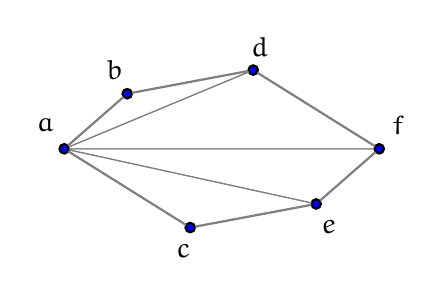
\begin{tikzpicture}[xscale=0.8]
\node at (-0.3,0.3) {$a$};
\node at (0.8,1) {$b$};
\node at (1.9,-1.3) {$c$};
\node at (3.1,1.3) {$d$};
\node at (4.2,-1) {$e$};
\node at (5.3,0.3) {$f$};
\node[draw,circle, thick, fill=blue, scale=0.3] (a) at (0,0) {};
\node[draw,circle, thick, fill=blue, scale=0.3] (b) at (1,0.7) {};
\node[draw,circle, thick, fill=blue, scale=0.3] (c) at (2,-1) {};
\node[draw,circle, thick, fill=blue, scale=0.3] (d) at (3,1) {};
\node[draw,circle, thick, fill=blue, scale=0.3] (e) at (4,-0.7) {};
\node[draw,circle, thick, fill=blue, scale=0.3] (f) at (5,0) {};
\draw[gray, thick] (a) -- (b) -- (d) -- (f) -- (e) -- (c) -- (a);
\draw[gray] (a) -- (b) -- (d) -- (a);
\draw[gray] (a) -- (c) -- (e) -- (a);
\draw[gray] (a) -- (e) -- (f) -- (a);
\draw[gray] (a) -- (d) -- (f) -- (a);
\end{tikzpicture}
\end{minipage}
}


\section{Progress and Conclusions}
\frame{\Large \tableofcontents[currentsection]}

\frame{
	\frametitle{Determined $6$-hole or $7$-gon}

\large

\begin{itemize}
\item Every set of $33$ points has likely a $7$-gon
\item Every set of $30$ points has likely a $6$-hole
\item How many points are required for a $7$-gon or $6$-hole? \pause \structure{24}
\end{itemize}

\bigskip
We partitioned the problem into 7821 subproblems:
\medskip


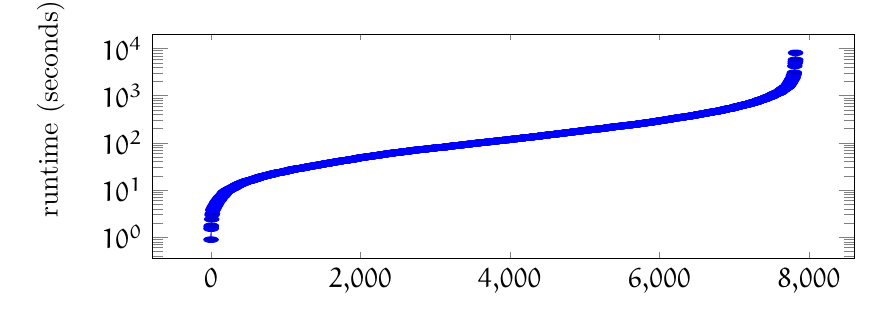
\begin{tikzpicture}
          \begin{axis}[ymode=log, yscale=0.5, xscale=1.3,ylabel={runtime (seconds)\!\!\!\!\!\!\!\!\!\!\!\!\!\!\!\!}]
          \addplot coordinates {(1,0.89) (2,1.52) (3,1.56) (4,1.70)(5,1.75) (10,2.41) (15,2.98) (20,3.20) (25,3.77) (30,3.89) (35,3.99) (40,4.16) (45,4.39) (50,4.50) (55,4.62) (60,4.74) (65,4.89) (70,5.08) (75,5.28) (80,5.40) (85,5.65) (90,5.74) (95,5.95) (100,6.01) (105,6.12) (110,6.26) (115,6.49) (120,6.62) (125,6.82) (130,6.98) (135,7.16) (140,7.27) (145,7.35) (150,7.49) (155,7.60) (160,7.83) (165,7.94) (170,8.08) (175,8.41) (180,8.55) (185,8.76) (190,8.98) (195,9.13) (200,9.23) (205,9.30) (210,9.39) (215,9.63) (220,9.75) (225,9.81) (230,9.91) (235,9.98) (240,10.04) (245,10.12) (250,10.34) (255,10.41) (260,10.53) (265,10.62) (270,10.73) (275,10.84) (280,10.89) (285,10.94) (290,11.13) (295,11.21) (300,11.24) (305,11.35) (310,11.50) (315,11.70) (320,11.77) (325,11.91) (330,12.01) (335,12.11) (340,12.25) (345,12.40) (350,12.55) (355,12.66) (360,12.80) (365,12.96) (370,13.01) (375,13.16) (380,13.25) (385,13.36) (390,13.49) (395,13.61) (400,13.67) (405,13.78) (410,13.84) (415,13.91) (420,14.12) (425,14.22) (430,14.29) (435,14.38) (440,14.58) (445,14.67) (450,14.82) (455,14.89) (460,14.98) (465,15.08) (470,15.17) (475,15.26) (480,15.33) (485,15.41) (490,15.53) (495,15.62) (500,15.73) (505,15.78) (510,15.82) (515,15.89) (520,15.96) (525,16.04) (530,16.09) (535,16.14) (540,16.20) (545,16.28) (550,16.37) (555,16.44) (560,16.53) (565,16.75) (570,16.94) (575,17.05) (580,17.13) (585,17.24) (590,17.32) (595,17.38) (600,17.42) (605,17.51) (610,17.63) (615,17.70) (620,17.85) (625,17.92) (630,18.13) (635,18.29) (640,18.38) (645,18.49) (650,18.65) (655,18.75) (660,18.80) (665,18.96) (670,19.06) (675,19.18) (680,19.22) (685,19.30) (690,19.36) (695,19.51) (700,19.58) (705,19.64) (710,19.75) (715,19.85) (720,19.89) (725,19.98) (730,20.08) (735,20.17) (740,20.31) (745,20.41) (750,20.50) (755,20.63) (760,20.68) (765,20.80) (770,20.93) (775,20.97) (780,21.05) (785,21.12) (790,21.18) (795,21.28) (800,21.32) (805,21.44) (810,21.52) (815,21.63) (820,21.76) (825,21.87) (830,22.01) (835,22.26) (840,22.36) (845,22.48) (850,22.61) (855,22.65) (860,22.74) (865,22.87) (870,22.95) (875,22.99) (880,23.04) (885,23.12) (890,23.23) (895,23.30) (900,23.35) (905,23.45) (910,23.54) (915,23.59) (920,23.67) (925,23.70) (930,23.84) (935,23.89) (940,23.94) (945,23.99) (950,24.08) (955,24.22) (960,24.34) (965,24.43) (970,24.48) (975,24.53) (980,24.70) (985,24.77) (990,24.91) (995,24.97) (1000,25.03) (1005,25.18) (1010,25.32) (1015,25.49) (1020,25.56) (1025,25.62) (1030,25.77) (1035,25.88) (1040,25.98) (1045,26.02) (1050,26.08) (1055,26.32) (1060,26.52) (1065,26.74) (1070,26.89) (1075,26.97) (1080,27.01) (1085,27.13) (1090,27.28) (1095,27.37) (1100,27.45) (1105,27.50) (1110,27.58) (1115,27.75) (1120,27.80) (1125,27.90) (1130,27.98) (1135,28.03) (1140,28.14) (1145,28.20) (1150,28.26) (1155,28.35) (1160,28.42) (1165,28.53) (1170,28.67) (1175,28.74) (1180,28.85) (1185,28.88) (1190,28.91) (1195,28.97) (1200,29.05) (1205,29.16) (1210,29.24) (1215,29.28) (1220,29.35) (1225,29.44) (1230,29.54) (1235,29.62) (1240,29.72) (1245,29.81) (1250,29.97) (1255,30.19) (1260,30.35) (1265,30.40) (1270,30.51) (1275,30.65) (1280,30.74) (1285,30.90) (1290,30.96) (1295,31.05) (1300,31.16) (1305,31.23) (1310,31.39) (1315,31.53) (1320,31.67) (1325,31.79) (1330,31.89) (1335,31.97) (1340,32.03) (1345,32.08) (1350,32.24) (1355,32.38) (1360,32.47) (1365,32.53) (1370,32.58) (1375,32.71) (1380,32.78) (1385,32.96) (1390,33.05) (1395,33.12) (1400,33.21) (1405,33.31) (1410,33.33) (1415,33.40) (1420,33.62) (1425,33.74) (1430,33.92) (1435,33.95) (1440,34.10) (1445,34.18) (1450,34.30) (1455,34.38) (1460,34.49) (1465,34.62) (1470,34.70) (1475,34.86) (1480,35.01) (1485,35.14) (1490,35.28) (1495,35.39) (1500,35.48) (1505,35.54) (1510,35.81) (1515,35.95) (1520,36.01) (1525,36.07) (1530,36.16) (1535,36.29) (1540,36.39) (1545,36.43) (1550,36.66) (1555,36.80) (1560,36.93) (1565,37.04) (1570,37.15) (1575,37.25) (1580,37.47) (1585,37.51) (1590,37.56) (1595,37.75) (1600,37.81) (1605,37.86) (1610,37.92) (1615,38.16) (1620,38.38) (1625,38.46) (1630,38.60) (1635,38.70) (1640,38.75) (1645,38.87) (1650,38.98) (1655,39.23) (1660,39.33) (1665,39.51) (1670,39.57) (1675,39.76) (1680,39.90) (1685,40.01) (1690,40.12) (1695,40.16) (1700,40.37) (1705,40.50) (1710,40.60) (1715,40.79) (1720,40.84) (1725,41.02) (1730,41.16) (1735,41.24) (1740,41.37) (1745,41.55) (1750,41.65) (1755,41.71) (1760,41.81) (1765,41.94) (1770,42.00) (1775,42.12) (1780,42.19) (1785,42.28) (1790,42.36) (1795,42.51) (1800,42.67) (1805,42.86) (1810,42.92) (1815,43.00) (1820,43.08) (1825,43.29) (1830,43.44) (1835,43.52) (1840,43.69) (1845,43.77) (1850,43.81) (1855,43.91) (1860,43.98) (1865,44.07) (1870,44.15) (1875,44.36) (1880,44.63) (1885,44.79) (1890,44.95) (1895,45.07) (1900,45.16) (1905,45.31) (1910,45.46) (1915,45.61) (1920,45.68) (1925,45.87) (1930,45.98) (1935,46.20) (1940,46.47) (1945,46.61) (1950,46.70) (1955,46.97) (1960,47.08) (1965,47.30) (1970,47.65) (1975,47.71) (1980,47.88) (1985,48.10) (1990,48.27) (1995,48.46) (2000,48.58) (2005,48.77) (2010,48.91) (2015,48.97) (2020,49.03) (2025,49.25) (2030,49.36) (2035,49.49) (2040,49.59) (2045,49.69) (2050,49.78) (2055,49.90) (2060,50.13) (2065,50.35) (2070,50.43) (2075,50.49) (2080,50.54) (2085,50.66) (2090,50.86) (2095,50.98) (2100,51.04) (2105,51.12) (2110,51.27) (2115,51.42) (2120,51.54) (2125,51.69) (2130,51.89) (2135,52.00) (2140,52.06) (2145,52.23) (2150,52.39) (2155,52.60) (2160,52.72) (2165,52.83) (2170,53.00) (2175,53.09) (2180,53.21) (2185,53.38) (2190,53.54) (2195,53.67) (2200,53.80) (2205,53.98) (2210,54.07) (2215,54.36) (2220,54.51) (2225,54.69) (2230,54.81) (2235,54.93) (2240,54.98) (2245,55.06) (2250,55.18) (2255,55.32) (2260,55.55) (2265,55.68) (2270,55.79) (2275,55.99) (2280,56.15) (2285,56.21) (2290,56.44) (2295,56.68) (2300,56.80) (2305,57.14) (2310,57.32) (2315,57.45) (2320,57.60) (2325,57.75) (2330,57.91) (2335,58.04) (2340,58.15) (2345,58.32) (2350,58.38) (2355,58.62) (2360,58.78) (2365,58.88) (2370,59.17) (2375,59.29) (2380,59.37) (2385,59.49) (2390,59.70) (2395,59.81) (2400,59.91) (2405,60.03) (2410,60.13) (2415,60.43) (2420,60.82) (2425,61.00) (2430,61.11) (2435,61.19) (2440,61.35) (2445,61.45) (2450,61.53) (2455,61.73) (2460,61.89) (2465,61.94) (2470,62.04) (2475,62.15) (2480,62.26) (2485,62.42) (2490,62.52) (2495,62.64) (2500,62.76) (2505,62.91) (2510,63.12) (2515,63.25) (2520,63.43) (2525,63.56) (2530,63.66) (2535,63.82) (2540,63.90) (2545,64.01) (2550,64.26) (2555,64.39) (2560,64.77) (2565,64.85) (2570,64.99) (2575,65.16) (2580,65.33) (2585,65.48) (2590,65.72) (2595,65.84) (2600,65.95) (2605,66.01) (2610,66.12) (2615,66.27) (2620,66.48) (2625,66.66) (2630,66.77) (2635,66.94) (2640,67.03) (2645,67.14) (2650,67.30) (2655,67.48) (2660,67.74) (2665,67.88) (2670,68.10) (2675,68.22) (2680,68.28) (2685,68.46) (2690,68.67) (2695,68.80) (2700,69.13) (2705,69.35) (2710,69.57) (2715,69.70) (2720,69.82) (2725,69.90) (2730,70.41) (2735,70.52) (2740,70.58) (2745,70.67) (2750,70.78) (2755,70.91) (2760,71.03) (2765,71.14) (2770,71.32) (2775,71.42) (2780,71.58) (2785,71.71) (2790,71.83) (2795,71.98) (2800,72.09) (2805,72.18) (2810,72.25) (2815,72.36) (2820,72.41) (2825,72.48) (2830,72.61) (2835,72.77) (2840,72.92) (2845,73.02) (2850,73.26) (2855,73.41) (2860,73.50) (2865,74.04) (2870,74.22) (2875,74.32) (2880,74.40) (2885,74.55) (2890,74.67) (2895,74.83) (2900,74.97) (2905,75.13) (2910,75.38) (2915,75.53) (2920,75.77) (2925,75.87) (2930,76.00) (2935,76.11) (2940,76.22) (2945,76.43) (2950,76.53) (2955,76.66) (2960,76.86) (2965,77.21) (2970,77.35) (2975,77.47) (2980,77.71) (2985,77.90) (2990,78.14) (2995,78.27) (3000,78.44) (3005,78.53) (3010,78.71) (3015,78.97) (3020,79.01) (3025,79.13) (3030,79.23) (3035,79.40) (3040,79.44) (3045,79.60) (3050,79.68) (3055,79.90) (3060,79.97) (3065,80.12) (3070,80.28) (3075,80.34) (3080,80.42) (3085,80.48) (3090,80.58) (3095,80.67) (3100,80.80) (3105,81.03) (3110,81.25) (3115,81.36) (3120,81.56) (3125,81.92) (3130,82.11) (3135,82.25) (3140,82.36) (3145,82.66) (3150,82.78) (3155,82.85) (3160,83.02) (3165,83.36) (3170,83.43) (3175,83.56) (3180,83.74) (3185,83.85) (3190,84.24) (3195,84.54) (3200,84.76) (3205,84.95) (3210,85.31) (3215,85.45) (3220,85.71) (3225,85.87) (3230,86.07) (3235,86.32) (3240,86.53) (3245,86.68) (3250,86.91) (3255,87.11) (3260,87.26) (3265,87.38) (3270,87.52) (3275,87.63) (3280,87.84) (3285,88.18) (3290,88.29) (3295,88.49) (3300,88.59) (3305,88.80) (3310,88.91) (3315,88.98) (3320,89.30) (3325,89.48) (3330,89.62) (3335,89.81) (3340,89.98) (3345,90.25) (3350,90.34) (3355,90.58) (3360,90.79) (3365,91.08) (3370,91.19) (3375,91.22) (3380,91.47) (3385,91.65) (3390,91.96) (3395,92.12) (3400,92.33) (3405,92.59) (3410,92.66) (3415,92.80) (3420,93.04) (3425,93.30) (3430,93.49) (3435,93.74) (3440,94.02) (3445,94.14) (3450,94.56) (3455,94.73) (3460,94.90) (3465,95.03) (3470,95.19) (3475,95.35) (3480,95.67) (3485,95.85) (3490,96.04) (3495,96.20) (3500,96.31) (3505,96.57) (3510,96.82) (3515,97.06) (3520,97.33) (3525,97.46) (3530,97.76) (3535,97.88) (3540,98.18) (3545,98.32) (3550,98.56) (3555,98.77) (3560,99.10) (3565,99.37) (3570,99.46) (3575,99.73) (3580,99.80) (3585,99.97) (3590,100.25) (3595,100.55) (3600,100.70) (3605,100.87) (3610,100.98) (3615,101.32) (3620,101.63) (3625,101.79) (3630,102.06) (3635,102.31) (3640,102.42) (3645,102.58) (3650,102.71) (3655,102.95) (3660,103.03) (3665,103.47) (3670,103.60) (3675,103.74) (3680,103.79) (3685,104.02) (3690,104.17) (3695,104.42) (3700,104.59) (3705,104.82) (3710,105.08) (3715,105.18) (3720,105.40) (3725,105.45) (3730,105.84) (3735,106.04) (3740,106.40) (3745,106.64) (3750,106.86) (3755,107.05) (3760,107.22) (3765,107.43) (3770,107.62) (3775,107.93) (3780,108.24) (3785,108.30) (3790,108.54) (3795,108.66) (3800,108.86) (3805,108.99) (3810,109.19) (3815,109.52) (3820,109.98) (3825,110.12) (3830,110.33) (3835,110.63) (3840,110.82) (3845,111.26) (3850,111.51) (3855,111.65) (3860,111.86) (3865,112.09) (3870,112.43) (3875,112.58) (3880,112.88) (3885,113.08) (3890,113.36) (3895,113.50) (3900,113.62) (3905,113.91) (3910,114.02) (3915,114.26) (3920,114.51) (3925,114.80) (3930,114.97) (3935,115.14) (3940,115.25) (3945,115.56) (3950,115.69) (3955,115.77) (3960,115.91) (3965,116.14) (3970,116.32) (3975,116.60) (3980,116.92) (3985,117.24) (3990,117.36) (3995,117.83) (4000,118.06) (4005,118.47) (4010,118.67) (4015,119.05) (4020,119.54) (4025,119.84) (4030,120.03) (4035,120.31) (4040,120.53) (4045,120.75) (4050,121.02) (4055,121.24) (4060,121.30) (4065,121.58) (4070,121.80) (4075,122.00) (4080,122.22) (4085,122.42) (4090,122.65) (4095,122.77) (4100,123.08) (4105,123.50) (4110,123.94) (4115,124.33) (4120,124.45) (4125,124.78) (4130,125.08) (4135,125.36) (4140,125.69) (4145,125.90) (4150,125.99) (4155,126.09) (4160,126.26) (4165,126.64) (4170,127.21) (4175,127.40) (4180,127.87) (4185,128.28) (4190,128.45) (4195,128.59) (4200,128.73) (4205,129.02) (4210,129.32) (4215,129.55) (4220,129.74) (4225,129.86) (4230,130.32) (4235,130.45) (4240,130.56) (4245,130.84) (4250,131.40) (4255,131.55) (4260,131.83) (4265,131.97) (4270,132.24) (4275,132.51) (4280,132.63) (4285,132.99) (4290,133.12) (4295,133.52) (4300,133.88) (4305,134.28) (4310,134.67) (4315,134.90) (4320,135.15) (4325,135.50) (4330,135.68) (4335,136.07) (4340,136.40) (4345,136.64) (4350,137.00) (4355,137.15) (4360,137.29) (4365,137.67) (4370,137.81) (4375,138.45) (4380,138.73) (4385,138.88) (4390,139.22) (4395,139.36) (4400,140.23) (4405,140.38) (4410,140.73) (4415,141.01) (4420,141.48) (4425,141.72) (4430,141.98) (4435,142.18) (4440,142.54) (4445,142.75) (4450,143.05) (4455,143.56) (4460,144.16) (4465,144.52) (4470,144.63) (4475,145.00) (4480,145.33) (4485,145.67) (4490,145.96) (4495,146.58) (4500,147.20) (4505,147.52) (4510,147.79) (4515,148.15) (4520,148.41) (4525,148.62) (4530,148.86) (4535,149.12) (4540,149.53) (4545,149.77) (4550,150.00) (4555,150.25) (4560,150.72) (4565,151.01) (4570,151.42) (4575,151.47) (4580,151.60) (4585,151.94) (4590,152.13) (4595,152.70) (4600,153.02) (4605,153.38) (4610,153.65) (4615,154.03) (4620,154.38) (4625,154.77) (4630,155.19) (4635,155.32) (4640,155.79) (4645,156.28) (4650,156.59) (4655,156.99) (4660,157.25) (4665,157.38) (4670,157.58) (4675,157.90) (4680,158.20) (4685,158.70) (4690,159.46) (4695,159.68) (4700,160.05) (4705,160.52) (4710,160.90) (4715,161.32) (4720,161.67) (4725,162.33) (4730,162.47) (4735,162.77) (4740,163.16) (4745,163.48) (4750,163.76) (4755,164.41) (4760,165.04) (4765,165.56) (4770,165.82) (4775,166.23) (4780,166.50) (4785,167.03) (4790,167.40) (4795,167.77) (4800,168.06) (4805,168.36) (4810,168.64) (4815,168.92) (4820,169.00) (4825,169.44) (4830,169.75) (4835,170.24) (4840,170.76) (4845,171.05) (4850,171.58) (4855,171.99) (4860,172.45) (4865,172.79) (4870,173.27) (4875,173.62) (4880,173.90) (4885,174.22) (4890,174.61) (4895,175.36) (4900,175.66) (4905,175.98) (4910,176.28) (4915,176.65) (4920,177.09) (4925,177.42) (4930,178.13) (4935,178.43) (4940,178.72) (4945,178.81) (4950,179.22) (4955,179.86) (4960,180.13) (4965,180.62) (4970,180.97) (4975,181.43) (4980,181.70) (4985,182.00) (4990,182.35) (4995,182.82) (5000,183.13) (5005,183.58) (5010,184.16) (5015,184.47) (5020,185.01) (5025,185.67) (5030,186.33) (5035,187.12) (5040,187.77) (5045,187.98) (5050,188.34) (5055,188.75) (5060,189.02) (5065,189.43) (5070,189.59) (5075,189.93) (5080,190.46) (5085,190.81) (5090,191.08) (5095,191.51) (5100,191.66) (5105,192.20) (5110,192.42) (5115,192.58) (5120,193.15) (5125,193.47) (5130,194.01) (5135,194.45) (5140,194.64) (5145,194.84) (5150,195.22) (5155,196.08) (5160,196.43) (5165,197.08) (5170,197.21) (5175,197.52) (5180,197.94) (5185,198.21) (5190,198.64) (5195,199.00) (5200,199.11) (5205,199.90) (5210,200.21) (5215,200.34) (5220,200.71) (5225,201.67) (5230,202.61) (5235,203.07) (5240,203.36) (5245,203.63) (5250,204.04) (5255,204.27) (5260,204.55) (5265,205.42) (5270,205.69) (5275,206.25) (5280,206.75) (5285,207.44) (5290,207.84) (5295,208.58) (5300,209.20) (5305,209.64) (5310,210.49) (5315,210.99) (5320,211.44) (5325,212.06) (5330,212.49) (5335,213.10) (5340,213.68) (5345,214.20) (5350,214.80) (5355,215.53) (5360,216.32) (5365,217.14) (5370,217.52) (5375,217.87) (5380,218.05) (5385,218.75) (5390,219.16) (5395,219.67) (5400,219.99) (5405,220.39) (5410,221.04) (5415,221.74) (5420,221.90) (5425,222.26) (5430,222.92) (5435,222.99) (5440,223.25) (5445,223.63) (5450,223.89) (5455,224.57) (5460,225.26) (5465,226.13) (5470,226.39) (5475,227.03) (5480,227.67) (5485,227.96) (5490,228.40) (5495,229.12) (5500,229.54) (5505,229.89) (5510,230.20) (5515,230.57) (5520,231.03) (5525,232.02) (5530,232.41) (5535,233.03) (5540,233.56) (5545,234.26) (5550,234.34) (5555,234.84) (5560,235.27) (5565,236.09) (5570,236.35) (5575,236.86) (5580,237.18) (5585,238.05) (5590,238.43) (5595,238.95) (5600,239.54) (5605,240.34) (5610,240.78) (5615,241.34) (5620,241.61) (5625,241.87) (5630,242.27) (5635,242.57) (5640,243.31) (5645,243.87) (5650,244.29) (5655,244.73) (5660,245.34) (5665,245.72) (5670,246.64) (5675,247.01) (5680,247.55) (5685,248.30) (5690,248.45) (5695,248.97) (5700,249.85) (5705,250.70) (5710,251.71) (5715,251.90) (5720,252.82) (5725,254.03) (5730,254.85) (5735,255.84) (5740,256.23) (5745,256.88) (5750,257.38) (5755,258.51) (5760,258.86) (5765,259.14) (5770,259.64) (5775,260.54) (5780,260.97) (5785,261.61) (5790,262.46) (5795,263.62) (5800,263.98) (5805,264.45) (5810,265.38) (5815,265.65) (5820,266.11) (5825,266.97) (5830,267.96) (5835,268.50) (5840,269.58) (5845,270.22) (5850,270.75) (5855,271.65) (5860,272.38) (5865,272.79) (5870,273.49) (5875,274.17) (5880,274.79) (5885,275.49) (5890,276.36) (5895,276.97) (5900,277.25) (5905,278.32) (5910,279.10) (5915,279.91) (5920,280.26) (5925,280.89) (5930,281.37) (5935,282.17) (5940,283.08) (5945,283.90) (5950,285.50) (5955,286.80) (5960,287.75) (5965,288.31) (5970,288.86) (5975,289.62) (5980,290.84) (5985,292.21) (5990,293.19) (5995,293.95) (6000,294.11) (6005,295.21) (6010,295.82) (6015,296.68) (6020,297.43) (6025,298.15) (6030,298.79) (6035,299.78) (6040,301.02) (6045,301.62) (6050,302.21) (6055,302.81) (6060,304.48) (6065,305.92) (6070,306.90) (6075,307.59) (6080,307.99) (6085,308.87) (6090,309.47) (6095,309.85) (6100,310.93) (6105,312.21) (6110,312.82) (6115,313.76) (6120,314.20) (6125,315.04) (6130,315.94) (6135,317.51) (6140,318.47) (6145,319.09) (6150,321.20) (6155,322.04) (6160,323.26) (6165,325.59) (6170,326.27) (6175,327.83) (6180,329.01) (6185,329.80) (6190,330.64) (6195,332.48) (6200,332.99) (6205,333.53) (6210,334.51) (6215,335.14) (6220,336.15) (6225,336.70) (6230,337.70) (6235,338.64) (6240,338.85) (6245,339.14) (6250,339.84) (6255,340.66) (6260,341.65) (6265,344.28) (6270,344.98) (6275,345.80) (6280,346.69) (6285,347.48) (6290,348.44) (6295,349.18) (6300,349.73) (6305,352.00) (6310,353.00) (6315,353.43) (6320,354.13) (6325,354.58) (6330,355.47) (6335,357.09) (6340,357.76) (6345,358.63) (6350,359.39) (6355,360.86) (6360,361.48) (6365,362.13) (6370,362.88) (6375,364.28) (6380,365.03) (6385,365.63) (6390,367.28) (6395,368.09) (6400,368.94) (6405,370.00) (6410,371.73) (6415,372.60) (6420,373.65) (6425,374.89) (6430,375.94) (6435,377.46) (6440,378.30) (6445,378.93) (6450,381.60) (6455,382.12) (6460,382.83) (6465,384.22) (6470,386.15) (6475,387.60) (6480,388.47) (6485,389.26) (6490,391.56) (6495,392.78) (6500,393.60) (6505,395.22) (6510,397.06) (6515,399.05) (6520,400.67) (6525,401.52) (6530,402.65) (6535,403.41) (6540,405.80) (6545,406.76) (6550,407.91) (6555,409.18) (6560,410.55) (6565,411.30) (6570,413.68) (6575,414.83) (6580,415.61) (6585,416.25) (6590,417.10) (6595,419.67) (6600,420.98) (6605,422.23) (6610,423.71) (6615,424.74) (6620,426.64) (6625,427.70) (6630,430.31) (6635,432.30) (6640,433.16) (6645,436.05) (6650,436.98) (6655,438.02) (6660,439.39) (6665,441.69) (6670,442.56) (6675,444.11) (6680,446.27) (6685,447.55) (6690,448.82) (6695,450.88) (6700,451.72) (6705,452.45) (6710,454.80) (6715,455.79) (6720,456.43) (6725,456.82) (6730,458.16) (6735,458.81) (6740,460.13) (6745,461.49) (6750,464.03) (6755,465.77) (6760,467.44) (6765,468.03) (6770,470.37) (6775,471.45) (6780,472.85) (6785,473.78) (6790,476.78) (6795,479.21) (6800,480.69) (6805,481.79) (6810,483.24) (6815,485.52) (6820,488.09) (6825,488.98) (6830,490.30) (6835,493.42) (6840,494.24) (6845,498.40) (6850,500.11) (6855,503.52) (6860,505.55) (6865,507.04) (6870,509.40) (6875,510.72) (6880,512.55) (6885,514.20) (6890,517.44) (6895,519.29) (6900,522.29) (6905,525.78) (6910,527.51) (6915,528.49) (6920,530.23) (6925,532.26) (6930,534.28) (6935,536.19) (6940,537.45) (6945,538.80) (6950,540.42) (6955,541.76) (6960,542.61) (6965,544.05) (6970,546.48) (6975,549.88) (6980,551.71) (6985,556.09) (6990,558.14) (6995,560.60) (7000,562.71) (7005,565.17) (7010,570.67) (7015,574.77) (7020,577.30) (7025,581.88) (7030,585.27) (7035,587.64) (7040,589.49) (7045,590.51) (7050,592.41) (7055,595.04) (7060,598.73) (7065,601.39) (7070,605.38) (7075,606.77) (7080,608.35) (7085,611.89) (7090,612.79) (7095,614.83) (7100,618.42) (7105,622.87) (7110,625.04) (7115,628.64) (7120,634.32) (7125,635.61) (7130,638.58) (7135,639.47) (7140,641.82) (7145,645.23) (7150,648.95) (7155,651.30) (7160,652.67) (7165,656.51) (7170,660.12) (7175,663.12) (7180,664.81) (7185,666.17) (7190,669.29) (7195,672.28) (7200,675.36) (7205,681.76) (7210,685.56) (7215,690.95) (7220,692.91) (7225,697.80) (7230,699.36) (7235,701.11) (7240,708.46) (7245,713.57) (7250,716.19) (7255,719.60) (7260,725.02) (7265,728.53) (7270,732.01) (7275,733.70) (7280,736.23) (7285,740.34) (7290,743.95) (7295,748.67) (7300,756.65) (7305,759.11) (7310,765.89) (7315,777.14) (7320,780.68) (7325,785.63) (7330,793.84) (7335,796.50) (7340,800.84) (7345,804.94) (7350,808.74) (7355,814.11) (7360,817.52) (7365,823.14) (7370,827.45) (7375,833.78) (7380,836.44) (7385,845.23) (7390,853.69) (7395,856.61) (7400,859.34) (7405,864.38) (7410,872.66) (7415,876.75) (7420,884.57) (7425,887.13) (7430,899.59) (7435,909.54) (7440,915.14) (7445,921.95) (7450,926.34) (7455,934.03) (7460,939.80) (7465,945.84) (7470,952.89) (7475,954.85) (7480,961.26) (7485,969.76) (7490,978.82) (7495,983.60) (7500,996.07) (7505,1000.46) (7510,1016.78) (7515,1032.61) (7520,1039.55) (7525,1054.33) (7530,1066.95) (7535,1072.41) (7540,1080.11) (7545,1087.27) (7550,1097.22) (7555,1105.42) (7560,1113.14) (7565,1126.18) (7570,1131.27) (7575,1135.21) (7580,1144.98) (7585,1149.09) (7590,1159.65) (7595,1171.39) (7600,1181.37) (7605,1197.50) (7610,1204.40) (7615,1214.98) (7620,1237.58) (7625,1261.81) (7630,1282.91) (7635,1296.78) (7640,1313.06) (7645,1333.46) (7650,1349.69) (7655,1367.99) (7660,1395.34) (7665,1402.54) (7670,1413.95) (7675,1445.41) (7680,1463.65) (7685,1482.68) (7690,1496.28) (7695,1511.78) (7700,1532.58) (7705,1542.98) (7710,1558.63) (7715,1589.26) (7720,1633.85) (7725,1676.34) (7730,1724.56) (7735,1769.00) (7740,1854.37) (7745,1866.43) (7750,1907.37) (7755,2009.32) (7760,2050.66) (7765,2143.07) (7770,2198.04) (7775,2270.57) (7780,2307.69) (7785,2397.99) (7790,2597.22) (7795,2759.86) (7800,2837.96) (7805,3082.90) (7810,4285.24) (7815,4898.23) (7820,5758.85) (7818,5318.54) (7819,5368.67) (7820,5758.85) (7821,8140.93)};
          
          \end{axis}
\end{tikzpicture}

%\pause

\medskip

Total runtime: 530 CPU hours 


	
}

\newtheorem{conjecture}[theorem]{\translate{Conjecture}}

\frame{
	\frametitle{Status of $6$-hole}
	
\large

\begin{conjecture}
$h(6) = 30$
\end{conjecture}

\bigskip \bigskip

Solving the only remaining hole problem is within reach
\begin{itemize}
\item Strong evidence that the conjecture holds
\item The heuristics for smaller problems are also effective
\item We randomly solved approximately 3\% of the search space
\item Rough estimation: 300,000 CPU hours solving + checking
\item Linear-time scaling with thousands of cores
\end{itemize}
	
}

\frame{
	\frametitle{Conclusions}
	
\large

SAT solving appears to be the most effective technology to 
reasoning about patterns that emerge in the plane

\bigskip
\bigskip

Several open problems can likely be solved in the foreseeable 
future, including the $6$-hole problem
\begin{itemize}
\item Would close the final question for holes
\item Would be the hardest problem solved using SAT
\item Will be using concurrent solving and checking
\end{itemize}
	
}


\end{document}
